\documentclass[sigconf,nonacm]{acmart}

%% packages
\usepackage{graphicx}
\usepackage{lipsum}
\usepackage{url}

%% header
\title{Arcadia Finance [Draft]}
\subtitle{November 2023}
\date{November 2023}

\author{Thomas Smets}
\affiliation{
    \institution{Arcadia Finance}
    \city{Brussels}
    \country{Belgium}
}
\email{thomas@arcadia.finance}

\renewcommand{\shortauthors}{Smets et al.}

%% Add whitespace under header
\begin{teaserfigure}
    \vspace{1em}
    \Description{Just used to add a whitespace over the length of the document.}
\end{teaserfigure}

%% Show page numbers
\settopmatter{printfolios=true}

%% Decrease whitespace under Figures
\setlength\textfloatsep{\baselineskip}

\begin{document}

\begin{abstract}
    Arcadia Finance introduces a novel on-chain architecture, the Arcadia Finance Technology Stack,
    designed for efficient collateral management of margined positions.

    As we anticipate the continued growth of tokenized assets and emergence of new on-chain financial primitives, 
    the importance of standardized and efficient collateral management becomes increasingly paramount.

    Arcadia strives to enable higher capital efficiency for users, transparent risk assessment,
    faster go-to-market time for new protocols and an improved user experience.
    All without compromising on security, self-custody and decentralization.
\end{abstract}

\keywords{Collateral Management, DeFi, Margin, EVM}

\maketitle

\section{Introduction} 
\label{sec:introduction}
This paper will explain the rationale behind the Arcadia Finance Technology Stack, what its main benefits are,
and how it is technically implemented (the latter starts from Section \ref{sec:arcadia-financial-technology-stack} onwards).

The Arcadia Financial Technology Stack is a set of on-chain, inter-linked financial protocols,
centered around collateral management and margined positions.
They facilitate non-trusting Debtors and Creditors to close financial contracts without the need of trusted intermediaries.

It consists of three protocols, each with distinct responsibilities and permissions:
\begin{itemize}
\item The Arcadia Registry.
\item The Arcadia Accounts.
\item The Generalized Creditor.
\end{itemize}

To establish a shared understanding, this paper starts with Section \ref{sec:terminology},
where concepts and terminology related to collateral management and margined positions are defined.

Section \ref{sec:collateral-managemen-in-traditional-finance} provides a brief exploration of the use of collateral in the traditional financial system.

Following this, Section \ref{sec:collateral-management-in-DeFi} goes into more detail on how collateral is used within DeFi,
pinpointing current shortcomings and inefficiencies, and discusses how novel architectures might address these issues.

In Section \ref{sec:arcadia-financial-technology-stack} our implementation of such a novel architecture is introduced:
the Arcadia Financial Technology Stack.

Finally, each of the underlying protocols of the Arcadia Financial Technology Stack is discussed in detail 
in Sections \ref{sec:arcadia-registry}, \ref{sec:arcadia-accounts} and \ref{sec:arcadia-creditor}.

\section{Terminology}
\label{sec:terminology}
\textsc{Collateral:} The assets pledged by a Debtor to a Creditor to cover the credit risk in case the Debtor would default.

\textsc{Debtors and Creditors:} The terms Debtors and Creditors are often used throughout this paper.
Our definition is broader than the commonly accepted context within traditional debt arrangements.
The term Debtor is used for any holder of a financial instrument that results in liabilities on the balance sheet
(borrowers, option writers, payers of cash-settled futures contract or swaps...).
The Creditor refers to the entity to whom the liability is owed.

\textsc{Margin:} The value of collateral assets that a Debtor must hold in a Margin Account to cover the credit risk of its Creditor(s).
The margin requirements, are set by the Creditor.
It is the value of assets that is "locked" when a Debtor opens a position.

\textsc{Margin Account:} Our definition of a Margin Account extends beyond the conventional usage within Brokerage Accounts.
A Margin Account is an account held by a Debtor that mitigates the counterparty risk, borne by the Creditor.
It does so by guaranteeing that the total value of all assets within the Account is always bigger than the liabilities owed to the Creditor.

\textsc{Open position:} The size of the liability that a specific Debtor has with a specific Creditor.

\section{Collateral Management in Traditional Finance}
\label{sec:collateral-managemen-in-traditional-finance}

Evidence of collateralized loans, also known as secured loans, can be traced back to at least 400 BCE in Ancient Greece \cite{millett2002lending}.
In these early transactions, borrowers provided tangible assets as collateral to secure loans, laying the foundation for the concept of collateralization.

With the rise of complex financial instruments and the globalization of markets, the role of collateral has expanded beyond traditional lending.
Collateral is now used to secure a wide range of financial instruments, including derivatives trading, margin accounts,
and other sophisticated financial contracts.

The digitalization of the financial system greatly improved the efficiency of the exchange and settlement of collateral.
Reporting, margining and reconciliation processes could be executed on a daily basis instead of on a weekly or even monthly basis \cite{simmons2019collateral}.

But collateralization in the traditional financial world is not without its problems.
The 2008 financial crisis highlights the need for better collateral management infrastructure.

Bad collateral management, rehypothecation of collateral, opaque accounting practices
and outright fraud with collateralized assets, are all cited as root causes\cite{hellwig2008causes} behind the 2008 financial crisis.
Following the crisis, a variety of major regulations were introduced (e.g. EMIR in the European Union, or Dodd-Frank in the USA).

While these packages were successful in stabilizing the financial system, they have clear centralisation tendencies\cite{gregory2014central}.
The major beneficiaries of said regulations are the major established institutions, mandatory intermediaries for central clearing,
central banks and the regulatory bodies themselves.
This might paradoxically cement even greater systemic risks into the financial system.

\section{Collateral Management in DeFi}
\label{sec:collateral-management-in-DeFi}

Blockchain has some excellent properties with regards to collateral management:
\begin{itemize}
    \item With its immutable and transparent ledger, collateral can be audited 24/7.
    \item Smart contracts enforce margin requirements real time on a 24/7 continuous basis.
    \item Atomic execution of transactions avoids expensive reconciliation processes and eliminates settlement risk.
    \item Atomic execution of transactions enables optimistic execution of transactions (e.g. flash loans),
    which can greatly improve processes such as refinancing liabilities or even enable completely new financial use-cases.
    \item The permissionless nature of blockchain and Dapps (Decentralized Applications),
    combined with a shared state between all those applications,
    make different financial applications and assets composable and inter-operable by default.
\end{itemize}

Hence it is not a coincidence that some of the first blockchain applications with product market fit, 
like Maker\cite{team2017dai}, Aave\cite{thornburg2020aave} or Compound\cite{leshner2019compound},
were collateralized lending protocols.

\subsection{General Principles}
Lending protocols are not the only DeFi protocols that use collateralization to mitigate counterparty risks between different user-groups in some way or shape.
Perpetual protocols, Prime brokerage protocols, option protocols etc. all require some or all users to deposit collateral.

Most of these DeFi protocols require their users to over-collateralize their open positions,
meaning that the sum of all collateralized assets must always be larger, with a certain safety margin,
than the sum of all liabilities.

For example, if users want to borrow \$800 worth of token A via a certain lending protocol,
they must first deposit and lock at least \$1000 worth of token B as collateral in said protocol.

Additionally, most protocols have some kind of liquidation mechanism in place to prevent bad debt when the market moves against a user's position.
Taking the previous example, if token B drops in value compared to token A, say from \$1000 to \$900,
the user's position can be (fully or partially) liquidated.



\subsection{Shortcomings and Inefficiencies}
\label{subsec:shortcomings-and-inefficiencies}

There are however still a number of shortcomings and inefficiencies which need to be overcome,
before DeFi can be broadly adopted as the go-to infrastructure for collateral management.

\subsubsection{Collateralized in Name Only}
In 2022 DeFi experienced its own financial crisis.
In a few months time, many of the ecosystem's key (albeit mostly centralized) players, and a number of protocols collapsed.
Again bad collateral management, rehypothecation of collateral, opaque protocol mechanisms,
and outright fraud with collateralized assets were at the root of the problem.

A recurring trend with protocols that imploded in 2021 and 2022 is that the lack of collateralization was obfuscated behind complex protocol designs and narratives. 
Some of the notorious examples are:
\begin{itemize}
    \item Synthetic stable-tokens such as Gaia-USDf, Iron-Titan and Luna-Terra.
    \item Olympus and its forks relying on the (3,3) model.
    \item Protocols where the only utility of a token is to receive more of the token itself (animal yield farms, reflective tokens…).
    \item Unsecured loans by market makers and CeFi players.
\end{itemize}

The over-collateralized DeFi protocols however, operated remarkably well during the aforementioned crisis, even better than their traditional counterparts.
This is well illustrated by some of the collapsed centralized entities, active in the space until 2022, that had both on- and off-chain liabilities.
All on-chain Creditors were repaid in a timely and orderly fashion, as enforced by their smart contracts.
While the lawsuits for the many off-chain Creditors are, at the time of writing this paper, still ongoing (and probably will be for many years).

It is for these types of crises that liabilities are secured in the first place.
DeFi protocols should focus more on collateralization, and less on complex tokenomics that obfuscate who ends up paying when things go bad.

\subsubsection{Hacks and Exploits}
\label{subsubsec:hacks-and-exploits}

A major problem in DeFi today is the number of hacks and exploits occurring.
The estimated amount of funds lost in 2023 due to exploits ranges from \$400M to \$1B.
There are many security related practices the sector as a whole should improve on,
but we want to highlight one specific factor contributing significantly to this problem.

As mentioned before, almost all DeFi protocols use collateralization in some way of form.
While the nature of the financial contracts may be very different for each of these protocols, they share a great amount of common logic:
\begin{itemize}
    \item Pricing of collateralized assets.
    \item Management (depositing, withdrawing...) of collateralized assets.
    \item Margin calculations.
    \item Management of asset-liability specific risk parameters.
    \item Margin calls and liquidations of risky positions.
    \item Settling bad debt.
    \item ...
\end{itemize}

Pricing of assets, management of assets and liquidation logic is complex, error prone and most mistakes easily lead to severe user losses.
Today all protocols implement these redundant, even for new versions of the same protocol.

Not only is this very costly in development and auditing time, the core logic is rewritten and re-deployed time and time again,
and with each new deployment new bugs can be introduced.

Being able to build on top of battle-tested code would benefit smart contract developers, protocols, users and the overall ecosystem.

\subsubsection{Fragmented and Isolated Collateral}
\label{subsubsec:fragmented-collateral}

Having a global shared state across applications and assets is often cited as one of the key advantages of blockchain over centralized financial infrastructures\cite{schar2021decentralized}.
This should open up a whole new solution space for Debtors to manage collateralized positions,
and might even enable a single Debtor to share its margin between non-trusting Creditors without intermediaries.

But if we look at the reality today, we must admit that traditional brokers and clearing houses offer more advanced capabilities for cross- and portfolio-margined positions,
compared to the state-of-the-art DeFi protocol,
and the average DeFi-user has assets fragmented and isolated across a multitude of protocols.

There are multiple underlying root causes why collateral in DeFi is still fragmented and under-utilized:
\begin{itemize}
    \item As mentioned in Section \ref{subsubsec:hacks-and-exploits},
    there is no shared collateral management layer, each protocol with collateral has their own non-standardized implementation.
    \item Protocols are build around a single specific asset type (eg. lending protocols for simple ERC-20 or for AMM LPs, or for NFTs). 
    Different asset types cannot be used within the same protocol to back a single position and emergence of new primitives/token standards requires migrations/new protocols.
    \item Blockchain is still a young technology, core non-financial infrastructure required for on-chain portfolio management
    (think Account Abstraction, intents or cross-chain messaging) is only recently developed or still in development. 
\end{itemize}

While isolated margin positions have their benefits (they isolate risks), they are not capital efficient.
The volatility of a portfolio of assets is always equal to, or lower than the weighted volatility of the individual assets
(assets losing in value can be compensated with assets increasing in value).

Having a lower volatility, reduces the number of rebalancing actions (and their fees), reduces the number of liquidations
and depending on the correlations between collateralized assets, the Creditor might use less strict margin requirement.

Fragmentation of assets not only results in capital inefficiencies, it also contributes to a challenging user experience,
more on that in Section \ref{subsubsec:end-user-complexity}.

\subsubsection{End User Complexity}
\label{subsubsec:end-user-complexity}

End-users do not "want" to manage collateral.
Rather, they want to optimize portfolios to achieve certain objectives (e.g. increase yield, delta hedging, diversify exposure to different protocols...).
Collateral management is a means to an end, it is not an activity most users enjoy doing.

End-user adoption will only increase outside of a niche bubble of tech enthusiasts if the technical complexities around collateral management are abstracted away.
Important note, abstracting away technical complexities should never come at a cost of hiding risks or relying on centralized and custodial solutions (as is too often the case).

As mentioned in the previous Section \ref{subsubsec:fragmented-collateral}, the bad user experience is partly due to the fragmentation of assets and positions.
Having a standardized collateral management layer with standardized dapps across different protocols would benefit all users.

Rebalancing portfolios often require multiple transactions per asset and per position.
For which the user today has to execute multiple sequential transactions per asset, instead a single transaction that rebalances the complete portfolio.

Lets take as example a user that wants to earn yield from his collateralized assets and get exposure to Liquid Staking Tokens (LSTs).
Since LST protocols introduce an additional layer of risk, they wants to diversify risks over 5 different LST service providers.
Assuming our user has wrapped Ethereum, they would need to do 10 transactions via multiple platforms (5 approvals and 5 swaps or 5 approvals and 5 staking actions).
Rebalancing said portfolio, or depositing it as collateral, would require another 5 to 10 transactions.
Not only is this time consuming, it also introduces additional operational risks, to name a few:
 \begin{itemize}
    \item Herstatt risk (settlement risk) due to changing markets before each leg of the action is settled.
    \item Increased risk of manual mistakes (fat fingers, bad slippage settings).
    \item Increased risk of falling victim phishing attacks on one of the platforms. 
\end{itemize}
With Account abstraction, all these different action can be bundled in a single atomic on-chain transaction.

Another abstraction is to let users define what they want, and provide them with the information (the calldata) how to do it.
Since most collateral management actions require interactions with multiple assets/protocols,
this abstraction can only be achieved after portfolios as a whole can be managed with a single atomic transaction.

At the time of writing this paper, the required infrastructure to enable both abstractions, is heavily debated within the broader ecosystem and multiple proposals are launched to standardize the infrastructure.
Most notable are the proposals for Account Abstraction (e.g. EIP-3074 and EIP-4337) and for Intent based architectures (e.g. EIP-7521)

Both abstractions are already successfully applied (albeit in a somewhat non-standardized form) within DeFi by Decentralized Exchanges, NFT-marketplaces and their aggregators.

\subsection{New Architectures}
\label{subsec:new-architectures}
Over the course of 2023, a number of interesting solutions were proposed by different protocols and stakeholders on how to build more robust decentralized financial systems.
Notable recent papers are from Uniswap V4\cite{adams2023uniswap}, Morpho\cite{gontier2023morpho} and Euler\cite{euler2023protocols}.

All mention similar concepts as the distinction between product and protocol, modularization of the protocol,
oracle agnostic implementations and explicitly separating the logic of the protocol in different layers,
where layers with different complexity evolve at different speeds.

Especially the last concept, to separate the logic in different layers, resonates with the long term vision of the Arcadia Finance team.
Different Logic layers of the financial stack, with different complexities should have different life-cycles and innovation timelines.
With the lowest most core component the slowest moving, while the upper user facing layers must evolve and adapt quick in response to ever changing markets.

A good practical example is uniswap V4,
where Uniswap Labs implements the underlying core mathematical logic for CLAMMs (Concentrated Liquidity Automated Market Makers).
Other teams can build in a permissionless manner on top of the Uniswap V4 protocol and develop feature rich and fast innovating DEXs (Decentralized Exchanges),
without the need and risks of redundantly implementing the complex maths related to concentrated liquidity.

Over-collateralized protocols would benefit from a similar architecture as well.
A shared standardized and permissionless layer with battle-tested logic for collateral management and margin calculations,
on top of which Creditors build their application specific financial contracts.
Fast moving, end-user facing features can be developed independently of the core logic.

This is exactly what we are building with the Arcadia Financial Technology Stack.

\section{The Arcadia Financial Technology Stack}
\label{sec:arcadia-financial-technology-stack}

The Arcadia Financial Technology Stack, illustrated in Figure \ref{fig:arcadia-financial-technology-stack},
is our answer to resolve the inefficiencies outlined in Paragraph \ref{subsec:shortcomings-and-inefficiencies}.
It is implemented for the Ethereum Virtual Machine (EVM) and consists of three protocols:

\begin{samepage}
    \begin{itemize}
        \item The Arcadia Registry.
        \item The Arcadia Accounts.
        \item The Generalized Creditor.
    \end{itemize}
\end{samepage}

\begin{figure}
    \centering
    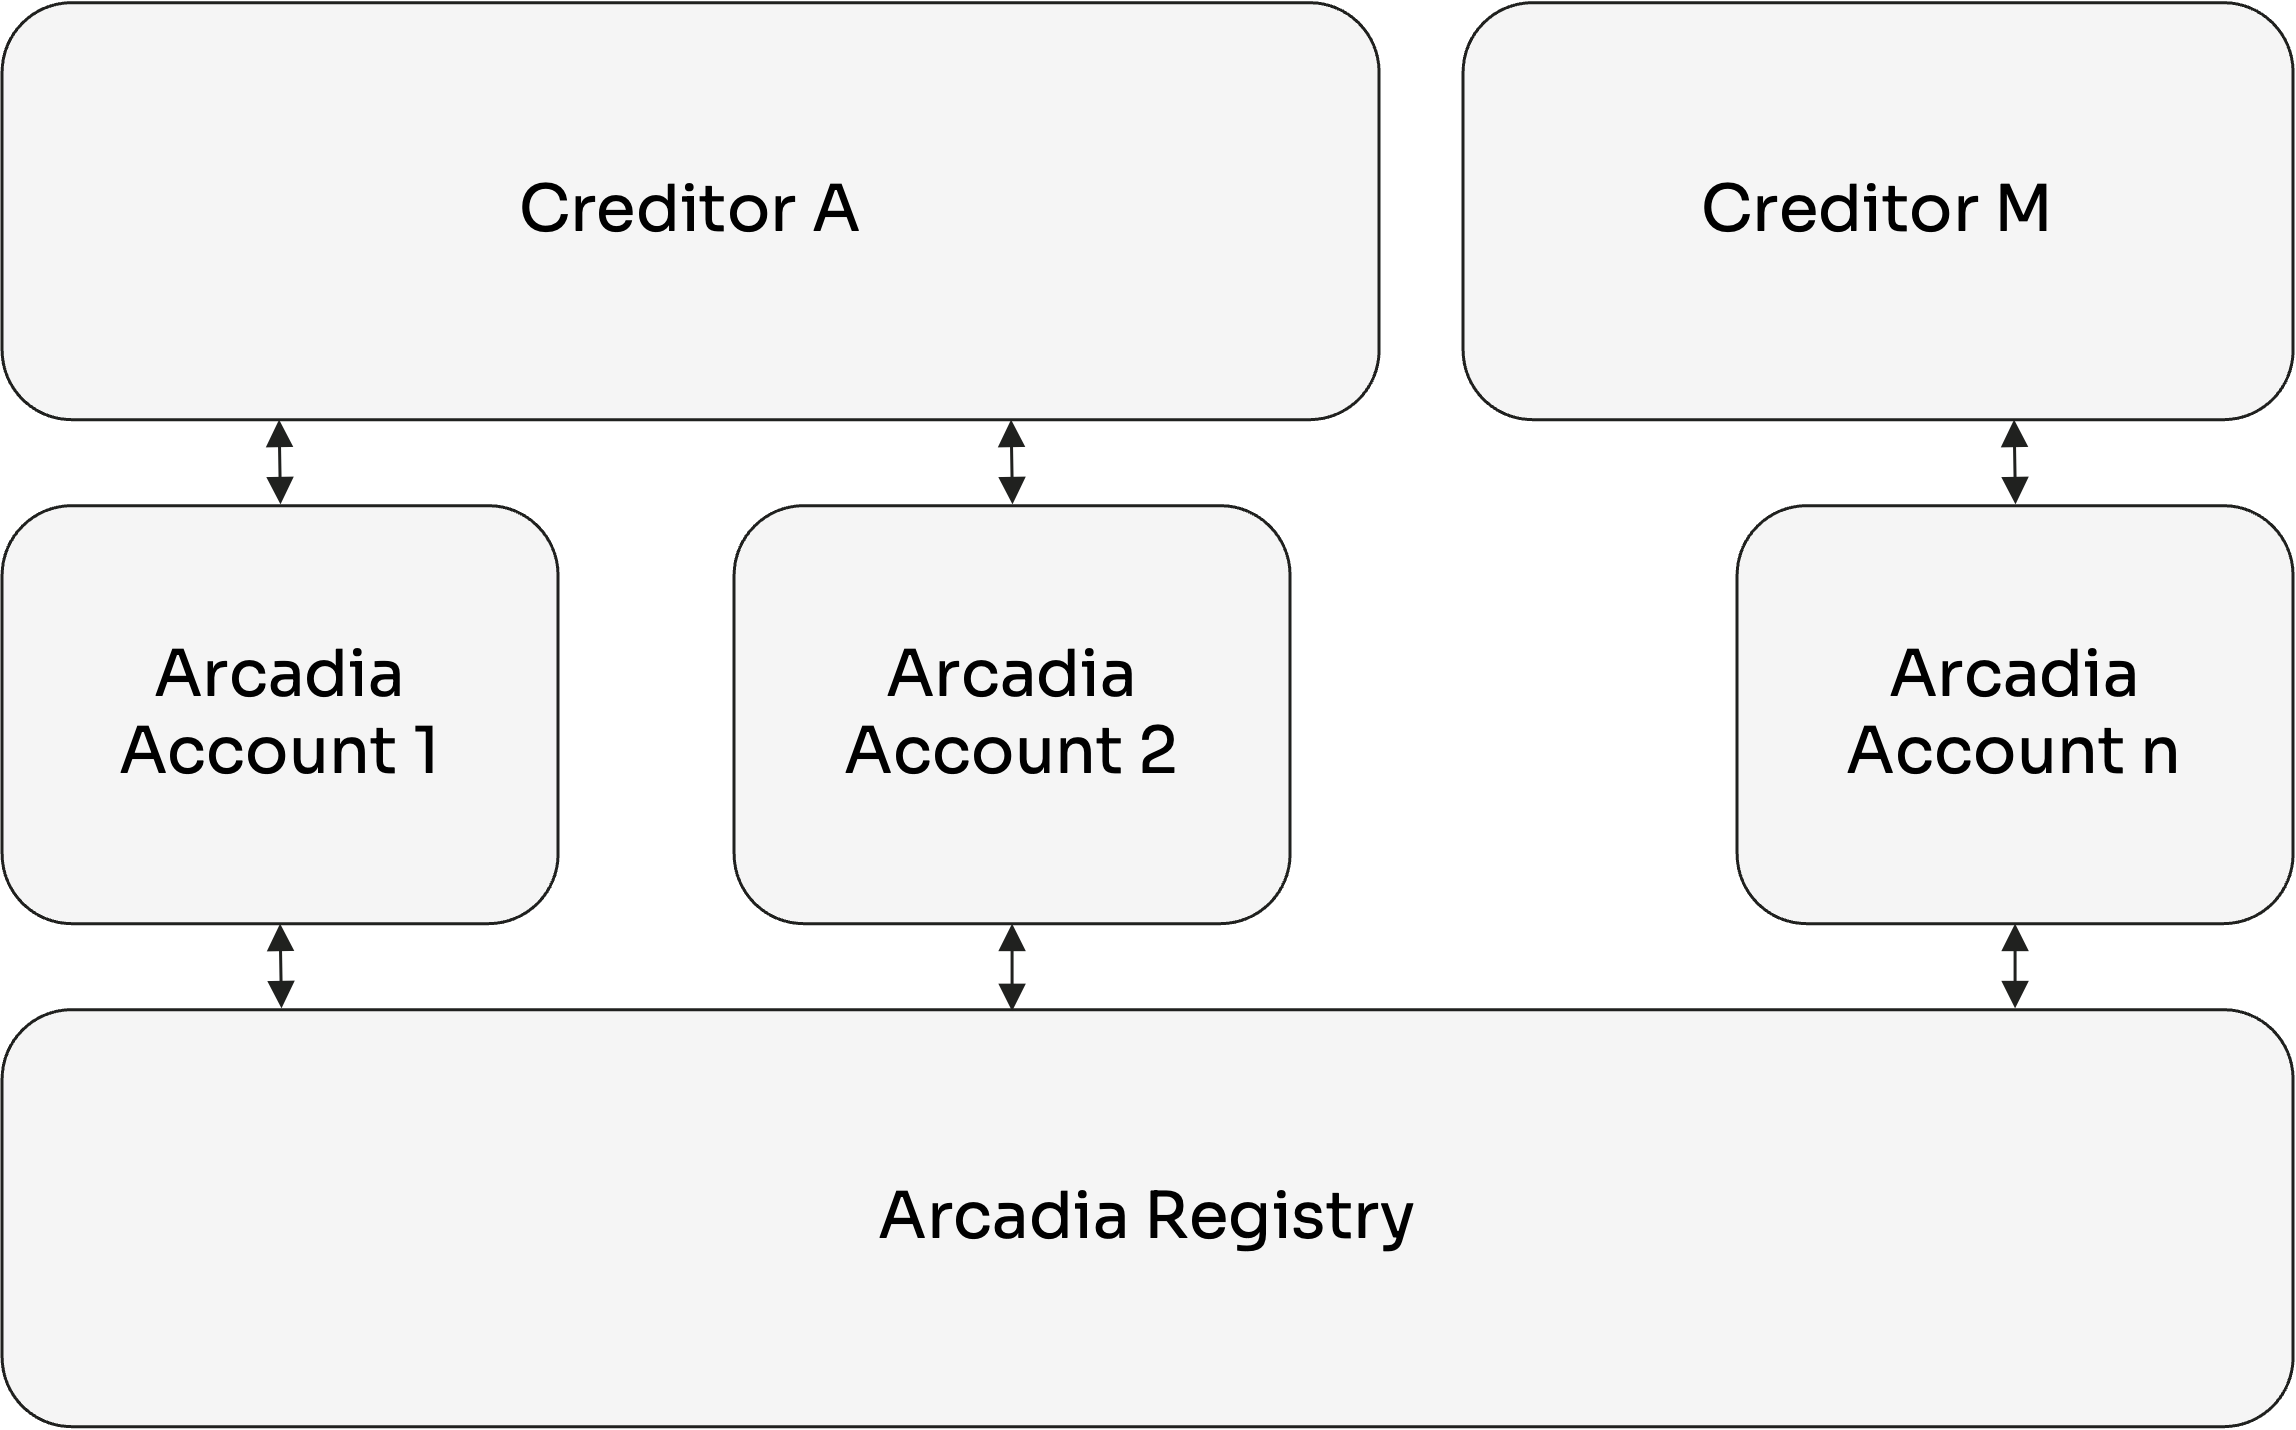
\includegraphics[width=0.45\textwidth]{images/Arcadia-Financial-Technology-Stack.png}
    \caption{The Arcadia Financial Technology Stack. \label{fig:arcadia-financial-technology-stack}}
    \Description{Shematic overview of the Arcadia Financial Technology Stack.}
\end{figure}

The Arcadia Registry is the least opinionated protocol and implements the core pricing and risk management logic.
By having a shared Arcadia Registry, Creditors can reuse battle-tested core logic.
This not only saves development time, but avoids that bugs are introduced in redundant implementations.

The Arcadia Accounts are advanced user-controlled smart wallets, responsible for asset management and enforcing the margin requirements of their owners.
With Arcadia Accounts, diversified portfolios can be used as collateral, and the same Account can serve as margin account for different Creditors.

Arcadia Accounts owners can batch together multiple account actions, automate account actions and interact optimistically with third party protocols.
Arcadia Accounts enable an unprecedented user experience, while not compromising on self-custody and composability.

Arcadia Accounts are further customable to suit specific needs of certain users or Creditors.

Lastly, the Generalized Creditor can be any protocol or financial contract where one or more users have liabilities, or can have liabilities at some point.
The protocol has to implement a single interface to become interoperable with the rest Arcadia Finance Technology Stack.

Protocols only have to implement their Creditor specific smart contracts,
and get the management of assets, pricing of assets, margin calculations... out of the box.

\subsection{L2 integration and Sequencer Stability}
\label{l2-integration-stability}

Within the Arcadia Finance Technology Stack, our commitment to technical robustness extends beyond traditional security measures, 
encompassing a forward-thinking approach to interoperability and resilience in the face of Layer 2 complexities. 
Our protocol is meticulously designed to be sequencer-ready, ensuring seamless integration with Layer 2 scaling solutions to enhance transaction 
throughput and reduce latency without compromising security. This readiness includes a proactive stance on potential disturbances in Layer 2 sequencers, 
such as sequencing risks, which are critical for maintaining uninterrupted service and user trust. 
We've implemented specific design choices and technologies that allow for efficient handling of these disturbances.
These integrations are pivotal in our strategy and reflecting our dedication to staying at the forefront of technological advancements.

\section{Arcadia Registry}
\label{sec:arcadia-registry}

The Arcadia Registry is non opinionated on-chain infrastructure with two main functionalities:
\begin{enumerate}
    \item Standardize pricing logic to denominate a portfolio of on-chain assets in a given numeraire (unit of account).
    \item Standardize logic to store, manage and process asset related risk parameters/variables.
\end{enumerate}

\subsection{Modular Pricing Logic}
\label{subsec:modular-pricing-logic}
The Arcadia Registry is not a monolithic smart contract containing all logic.
It consists of a main coordinating smart contract (also referred to as The Registry) and multiple append-only Modules.

Each Module is a separate smart contract with the pricing logic for specific Oracle implementations or specific Asset types.
The Registry keeps mappings per Creditor of which Module to use for a certain asset.

It is the Creditor itself that sets these mappings. The Creditor decides which Modules to use for each asset they allow their Debtors to use as collateral.
Different Creditors can use different Modules to price the same asset, or a Creditor can choose to not allow certain assets at all.

Modules can only be appended to the Registry, not removed or overwritten.
This ensures that Pricing logic is immutable, but it still gives flexibility to add new assets, or implement more efficient Pricing logic over time.

Working with this modular architecture has a number of advantages:
\begin{itemize}
    \item Modules are re-usable by different Creditors, instead of redundant monolithic Pricing Contracts per Creditor, battle-tested Pricing/Risk logic can be reused.
    \item Different Modules can call each other recursively, creating Pricing/Risk logic that is as composable as tokenized assets.
    \item Logic for new assets, or even asset types, can be added without the need of upgradable Proxy contracts and their inherent trust assumptions.
\end{itemize}

There are two main categories of modules: Oracle Modules and Asset Modules.
Asset Modules can be further divided in two sub-categories: Primary Asset Modules and Derived Asset Modules.
An overview of the different modules, and their relations are illustrated in Figure \ref{fig:arcadia-registry}.

\begin{figure}
    \centering
    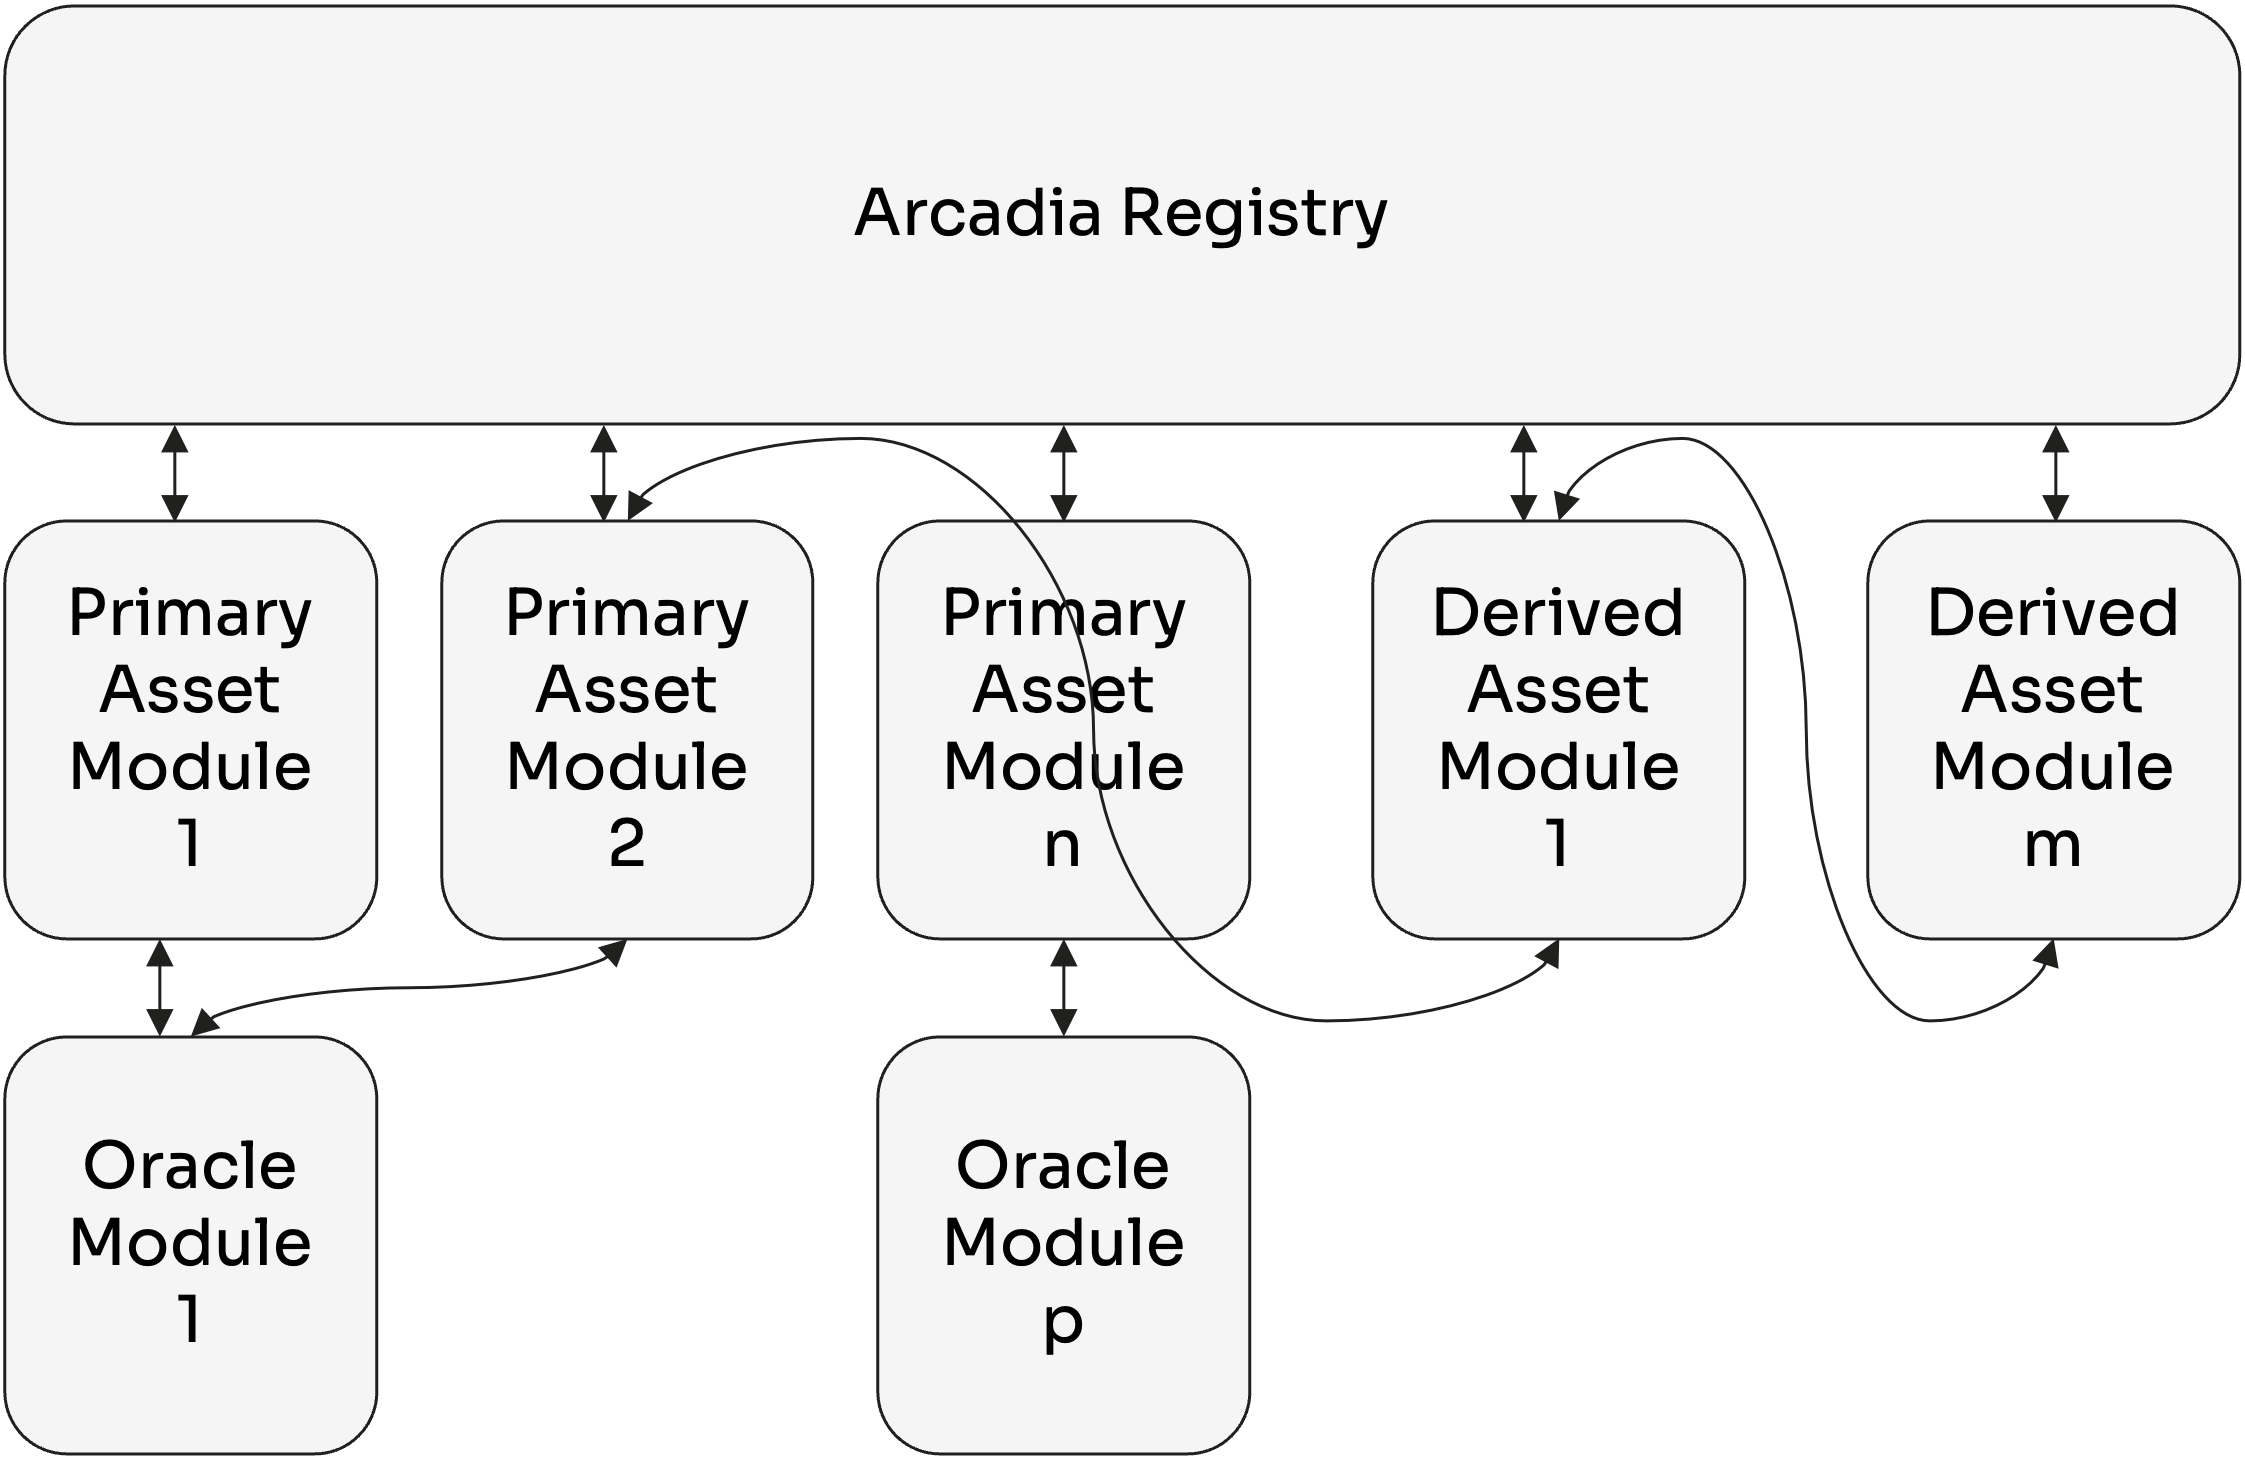
\includegraphics[width=0.45\textwidth]{images/Arcadia-Registry.png}
    \caption{The Arcadia Registry and Modules. \label{fig:arcadia-registry}}
    \Description{Shematic overview of the Arcadia Registry.}
\end{figure}

\subsection{Oracle Modules}
The Oracle Module implements the logic to convert oracle-rate of different oracle technologies into a standardized format.
Each different oracle implementation (e.g. Chainlink oracles, Pyth oracles, Uniswap TWAPs...) has its own Oracle Module.

Every oracle has a quote-asset and a base-asset, the oracle-rate $r_{oracle}$ reflects how much tokens of the quote-asset are required to buy 1 token of the base-asset.
The precision $S_{oracle}$ of oracles is variable and can even be a binary fixed-point number.
Since all pricing logic within the Arcadia Protocol uses fixed-point numbers with 18 decimals precision,
a correction from the oracle precision to a precision of 18 decimals is required for the standardized oracle rate $r_{ba\rightarrow qa}$, returned by the Oracle Module.
\begin{equation}
    \label{eq:oracle-module}
    r_{ba\rightarrow qa} = r_{oracle} \frac{10^{18}}{S_{oracle}}
\end{equation}

\subsection{Asset Modules}
Just as Oracle Modules implement the logic to return oracle-rates in a standardized format,
Asset Modules will return Asset values in a standardized format.
Similarly to how each oracle implementation has its own oracle Module, each asset type has its own Asset Module.

Next to pricing logic, Asset Modules also store and manage asset specific risk parameters, which we will discuss in more detail in Paragraph \ref{subsec:creditor-specific-cisk-parameters}.

Asset Modules can be further divided into two distinct groups: Primary Asset Modules and Derived Asset Modules.

\subsubsection{Primary Asset Modules}
Primary assets are defined as assets that are not composed of other assets.
Primary Assets must be priced using one or more on-chain oracles, for which the rates $r_{ba\rightarrow qa}$ are fetched from the Oracle Modules via the Registry.

The Primary Asset Modules will denominate all values of their assets in USD with 18 decimals precision.
Since the asset amount, $a_{asset}$, can have a variable precision (number of decimals),
a correction $S_{asset}$ is again applied to bring the USD value of the Primary Asset, $v_{asset}^{usd}$, to 18 decimals precision.

Depending of the direction of the oracle, the value of the Primary Asset is calculated differently.
When the asset is the base-asset of the oracle:
\begin{equation}
    v^{usd}_{asset}(a_{asset}) = r_{asset\rightarrow usd} \frac{a_{asset}}{S_{asset}}
\end{equation}

When the asset is the quote-asset of the oracle:
\begin{equation}
    v^{usd}_{asset}(a_{asset}) = \frac{1}{r_{usd\rightarrow asset}} \frac{a_{asset}}{S_{asset}}
\end{equation}

For some assets, there might not be a direct oracle to USD.
For these assets, multiple oracles can be chained together:
\begin{equation}
    v^{usd}_{asset}(a_{asset}) = r_{asset\rightarrow x} r_{x\rightarrow usd} \frac{a_{asset}}{S_{asset}}
\end{equation}
\begin{equation}
    v^{usd}_{asset}(a_{asset}) = \frac{r_{y\rightarrow usd}}{r_{y\rightarrow asset}} \frac{a_{asset}}{S_{asset}}
\end{equation}

\subsubsection{Derived Asset Modules}
Derived Assets are defined as assets that are composed of one or more underlying assets (which can be Primary Assets or other Derived Assets).
Examples of Derived Assets are liquidity positions of AMMs, staked assets, yield bearing tokens.

The Derived Asset Modules will calculate the USD value in three steps.
It will first calculate the amounts of the underlying assets $a_{u}$, given the amount of the asset to be priced $a_{asset}$.
\begin{equation}
    \label{eq:underlying-asset-amounts}
    a_{u} = f_{u}(a_{asset})
\end{equation}
Where $f_{u}(a)$ is a flashloan-resistant and protocol specific function.
For example for a Uniswap V2 Liquidity Positions it can be derived from the reserves of the Uniswap V2 pool contract,
or for ERC-4626 tokens it can be calculated by calling \texttt{convertToAssets(shares)}.

In a second step, the Derived Asset Module will recursively fetch the USD value of each of the underlying assets $v^{usd}(a_{u})$ from the Registry,
using the underlying asset amounts $a_{u}$ from Equation \ref{eq:underlying-asset-amounts}.
\begin{equation}
    v^{usd}(a_{u}) = v^{usd}(f_{u}(a_{asset}))
\end{equation}
The underlying assets of a Derived Asset can be Derived Assets themselves (e.g. staked LP tokens, or liquidity positions of AMMs where one of the tokens is a yield bearing asset).
In this case, the underlying asset will in turn fetch the USD values  of their underlying asset(s) recursively.
The stop condition of the recursion is when the underlying asset is a Primary Asset, or if a maximum recursion depth (set by the Creditor) is reached.

By working with modular and recursive Asset Modules, the pricing logic of the Registry fully captures the benefits of composability withing DeFi.

Lastly, the total USD value of the asset, $v^{usd}(a_{asset})$, is calculated as the sum of the USD values of its underlying assets.
Since all underlying assets are valued with 18 decimals precision, no additional precision correction is required.
\begin{equation}
    v^{usd}(a_{asset}) = \sum_{u}{v^{usd}(a_{u})} = \sum_{u}{v^{usd}(f_{u}(a_{asset}))}
\end{equation}

\subsection{Portfolio Pricing}
\label{subsec:portfolio-pricing}
Section \ref{subsec:modular-pricing-logic} explains how the Registry can calculate the value of assets in USD.
Building further on this logic, the Registry can price any combination of assets in any numeraire (the asset used as unit of account).

Given a portfolio $P$ consisting of assets with amount $a_{i}$, the value of the portfolio denominated in a certain numeraire $v_{spot}^{num}(P)$ is given as:
\begin{equation}
    \label{eq:portfolio-value-mtm}
    v_{spot}^{num}(P) = \frac{\sum_{i}{v^{usd}_{i}(a_{i})}}{r_{num\rightarrow usd}}\frac{S_{num}}{10^{18}}
\end{equation}
A correction $S_{num}$ is applied to bring the value from the 18 decimals precision to the actual decimal precision of the numeraire.

The result of equation \ref{eq:portfolio-value-mtm} is the spot or MtM (mark-to-market) value of the portfolio.

Next to the MtM value of the portfolio, the Registry can also calculate risk adjusted portfolios values,
where assets are discounted with a asset-Creditor specific risk factor $RF_{i}^{c}$, set by each Creditor.
The risk adjusted portfolio value $v_{risk}^{num}(P)$ is then given as:
\begin{equation}
    \label{eq:portfolio-value-risk-adjusted}
    v_{risk}^{num}(P) = \frac{\sum_{i}{RF_{i}^{c} \cdot v^{usd}_{i}(a_{i})}}{r_{num\rightarrow usd}}\frac{S_{num}}{10^{18}}
\end{equation}

There are two important risk adjusted portfolios values: The Collateral Value $v_{coll}^{num}$ of the Account and the Liquidation Value $v_{liq}^{num}$ of the account.

Both are used to check the Margin Requirements of the account.
The Collateral Value can be calculated by plugging the asset-Creditor specific Collateral Factors $CF_{i}^{c}$ of each asset into equation \ref{eq:portfolio-value-risk-adjusted}.
And the Liquidation Value respectively by using the Liquidation Factors $LF_{i}^{c}$ of each asset.

The Margin requirements, Collateral Value and Liquidation Value are discussed in more detail in Paragraph \ref{subsec:margin-accounts}.

\subsection{Creditor Specific Risk Parameters}
\label{subsec:creditor-specific-cisk-parameters}
Each Creditor can set a number of risk parameters in the Registry to protect themselves against different risks.
These risk parameters are taken into account when depositing assets, or when risk-adjusted portfolio values are calculated.

The risk parameters can be asset specific, protocol specific or a single value per Creditor.

\subsubsection{Collateral, Liquidation and Risk Factors}
As is described in detail in Paragraph \ref{subsec:margin-accounts}, Collateral Factors and Liquidation Factors are used to discount asset values to account for market, liquidity and smart-contract risks.

Each asset $i$ that can be priced by the Registry has a Creditor-specific Collateral Factor $CF_{i}^{c}$ and Liquidation Factor $LF_{i}^{c}$.
For Primary Assets, the factors are set directly by Creditor.

For Derived Assets, the risk factors are a function of the risk factors of its underlying assets $u$, and optionally an additional protocol specific risk factor $RF_{p}^{c}$,
to account for the additional complexity and smart contract risks of Derived Assets:
\begin{equation}
    CF_{i}^{c} = f(\forall CF_{u}^{c}, RF_{p}^{c})
\end{equation}

The relation between the risk factor of the Derived Asset and the risk factors of the underlying assets,
will depend on the specific nature of the Derived Asset.
It can be the minimum of each of the risk factors of the underlying assets, or a weighted average or something else.

For Derived Assets with a single underlying asset,
the risk factor becomes straightforward and is just the multiplication of the risk factor of the underlying asset and the protocol specific risk factor.
As an example, take a protocol ($p$) with yield bearing assets, which has an $ETH$ and a $USDC$ vault.
The Collateral Factors of the corresponding $pETH$ and $pUSDC$ tokens are:
\begin{equation}
    CF_{pETH}^{c} = RF_{p}^{c} \cdot CF_{ETH}^{c}
\end{equation}
\begin{equation}
    CF_{pUSDC}^{c} = RF_{p}^{c} \cdot CF_{USDC}^{c}
\end{equation}

\subsubsection{Maximum Exposure}
The maximum exposures give Creditors a tool to set upper boundaries against the overall exposures they can have against certain Primary Assets or protocols of Derived Assets.
Creditors can even choose to not be exposed to certain Primary Assets or protocols (via Derived Assets) by setting the corresponding maximum exposure to 0.

There is again a difference how the maximum exposure is defined for Primary Assets and for Derived Assets.

For Primary Assets, the maximum exposure is defined per Primary Asset and per Creditor.
It limits the total amount (in the unit of the underlying asset) of exposure that a single Creditor can have against the Primary Asset.
As such assets with low on-chain liquidity or small market caps can be used as collateral,
while market manipulation risks, such as the Mango Market Exploit\cite{coindeskDeFiExchange} can be mitigated.

The total exposure of a Primary Asset takes into account both direct deposits of the Primary Asset, as indirect exposures via Derived Assets.

If a maximum exposure is reached, no additional amount of the Primary Asset can be deposited,
nor can any Derived Asset be deposited that is composed of the Primary Asset.

For Derived Assets, there are two mechanisms that provide the Creditor to an upper bound for certain risks.
As mentioned before, none of the Primary Assets of which the Derived Asset is ultimately composed of, can exceed their maximum exposure to mitigate risks of market manipulation and low liquidity.
Secondly, each Creditor can set an upper limit to the total USD exposure of all Derived Assets of a certain protocol (e.g. the sum of all liquidity position of Uniswap V3).
As such, the Creditor can limit potential losses due to exploits in the protocol.

\subsubsection{Minimum Margin}
\label{subsubsec:minimum-margin}
Liquidating unhealthy positions has a considerable gas cost, which liquidators take into account when deciding to liquidate a position or not.
This gas cost is largely independent of the size of the open position.
Without a Minimum Margin, this could lead to very small unhealthy positions that are never profitable to liquidate.
Or even worse, liquidations that are successfully started, but never profitable to end.

To avoid both problems, Accounts must have a Creditor-specific minimum value of collateral, the minimum margin $M_{min}^c$, before they can open a position.
The minimum margin can not be used to back liabilities and can be seen as an amount of collateral that is locked to at least cover gas costs of Liquidators.

\section{Arcadia Accounts}
\label{sec:arcadia-accounts}
Arcadia Accounts serve as an advanced user-controlled smart wallet from which the owner can perform a multitude of actions: deposit and withdraw assets,
use the assets to interact with other DeFi protocols, open a margin account with a Creditor, open positions with the Creditor,
change from Creditor or transfer the Account to another owner.

Each Arcadia Account is a separate smart contract, owned by one single user.
Users can deploy one or more Accounts through the Arcadia Factory, ensuring the Account adheres to the source code as developed by the Arcadia team.

\subsection{Margin Accounts}
\label{subsec:margin-accounts}
Arcadia Accounts are more than the standard smart contract wallets, they can be used as on-chain Margin Accounts.
They are an extension to a smart contract wallet in a similar way to how a credit card is an extension to a debit card:
The owner of the account/card not only has control over the assets held by the account/card,
they can also use the account/card to incur liabilities.

Unlike credit cards however, Margin Accounts do not rely on trust and reputation to ensure liabilities are paid back.

The Margin Account mitigates the counterparty risk, borne by the Creditor,
by guaranteeing that the total value of all assets within the Account is always bigger than the liabilities against the Account (it is over-collateralized):
\begin{itemize}
    \item It holds the collateral assets and open positions of the Debtor (the Account owner).
    \item It does the accounting of both the assets and liabilities.
    \item It enforces the margin requirements continuously:
    \begin{itemize}
        \item Any Account Action that would bring it at risk of becoming under-collateralized is automatically reverted.
        \item If over time, due to changing values of assets/liabilities, it is at risk of becoming under-collateralized, a margin call is triggered.
    \end{itemize}
\end{itemize}

With Arcadia Accounts, the asset management, Accounting logic, and the enforcement of the margin requirements are 100\% implemented on-chain.
Arcadia Accounts are permissionless and fully composable with tokens and external DeFi protocols.
They can be used by on-chain investors to increase their buying power, to short assets, or to hold financial contracts such as futures, swaps, options or other derivatives.

In the next paragraphs we will introduce some margin related concepts and express the Margin requirements mathematically.

Note that we do not 100\% follow the conventions and terminology of the traditional financial world.

\subsubsection{Portfolio Margin}
Arcadia Accounts use portfolio margin calculations by default for their risk and margin calculations.

Portfolio margin has a number of advantages over isolated margin (where collateral is not shared between positions at all).
It is more capital efficient and prevents unnecessary liquidations or rebalancing of positions, leading to lower fees and potential losses.

Users that still want to have isolated positions can still do so by deploying multiple Accounts and depositing a single asset as collateral in each Account.

Portfolio margin is similar to cross-margin in that all assets bought on margin share the same collateral.
But unlike with cross-margin, there is no distinction between realized and unrealized profits.
Wins of one position offset losses of other positions, independent if they are realized or not,
making Portfolio margin even more capital efficient.

This is because Accounts do not make a distinction between the assets initially deposited as collateral and the assets bought on margin.
All assets held by the Account (deposited and bought) are taken in consideration for the margin calculations.

\subsubsection{Available Margin}
\label{subsubsec:available-margin}
We define the available margin, $am$, as the total value that the Account can use as margin to secure liabilities.

This total value equals the risk-adjusted portfolio value, expressed by Formula \ref{eq:portfolio-value-risk-adjusted},
where each asset is discounted with an asset-Creditor specific risk factor (the Collateral Factor).

Hence the available margin equals the Collateral Value as defined in Paragraph \ref{subsec:portfolio-pricing}
(we will use the terms 'available margin' and 'Collateral Value' interchangeable).
\begin{equation}
    \label{eq:available-margin}
    am := v_{coll}^{num} = \frac{\sum_{i}{CF_{i}^{c} \cdot v^{usd}_{i}(a_{i})}}{r_{num\rightarrow usd}}\frac{S_{num}}{10^{18}}
\end{equation}

\subsubsection{Open position}
The open position, $op^c$, equals the size of the liability that a specific Debtor has with a specific Creditor.

\subsubsection{Minimum Margin}
As explained in Paragraph \ref{subsubsec:minimum-margin}, the minimum margin, $M_{min}^c$, 
is the minimum amount of Collateral Value that must be held in an Account to be able to open position with a Creditor.

\subsubsection{Used Margin}
The used margin, $um$, is the total amount of Collateral Value locked by the Account to ensure that the Account remains over-collateralized.

Since collateral in the Account must be held to cover both the open position and the minimum margin, the used margin can be found as:
\begin{equation}
    um := M_{min}^c + op^c
\end{equation}

\subsubsection{Free Margin}
The free margin, $fm$, is the remaining amount of Collateral Value that can be used to increase the open position or that can be withdrawn from the Account's assets.

The free margin can be found by subtracting the used margin from the available margin:
\begin{equation}
    \label{eq:free-margin}
    fm := am - um
\end{equation}

\subsubsection{Initial Margin}
\label{subsubsec:initial-margin}
The initial margin of an asset, $IM_{i}^{c}$, is defined in the traditional financial world as the percentage of the value of an asset bought on margin (bought with debt)
that must be covered by additional collateral held in the Account at the time of the sale.

As an example, take an asset with an initial margin of 5\%, if someone want to buy 10,000 worth of the asset on margin,
they need to hold at least an additional 500 worth of collateral in their margin account.

The astute reader will see the similarities with the available margin and Collateral Factors as defined in Paragraph \ref{subsubsec:available-margin}.
There is indeed a mathematical relationship between the two.

Take an asset $i$, for which an amount of $x$ is bought on margin from Creditor $C$.
If a value of $x$ is borrowed, then at least a value of $IM_{i}^{c} \cdot x$ must be deposited as collateral into the Account.
The Account now has an open position of $x$ and holds in total $x + IM_{i}^{c} \cdot x$ of the asset $i$ ($IM_{i}^{c} \cdot x$ deposited as collateral and $x$ borrowed from Creditor $C$):
\begin{equation}
    \label{eq:initial-margin}
    \begin{split}
        &op^c = x\\
        &v^{num}_i = x + IM_{i}^{c} \cdot x
    \end{split}
\end{equation}

When the minimal amount of collateral is deposited, the free margin will be zero, and after plugging Equation \ref{eq:available-margin} into \ref{eq:free-margin}, the used margin equals the Collateral Value:
\begin{equation}
    CF_{i}^{c} \cdot v^{num}_i = um
\end{equation}
And if we ignore the minimum margin (which will be small compared to the open position in most cases) this simplifies to:
\begin{equation}
    CF_{i}^{c} \cdot v^{num}_i = op^c
\end{equation}
Finally after plugging in Equations \ref{eq:initial-margin}, we find the relation between the initial margin and the Collateral Factor:
\begin{equation}
    CF_{i}^{c} = \frac{1}{1 + IM_{i}^{c}}
\end{equation}

\subsubsection{Maintenance Margin}
The maintenance margin of an asset, $MM_{i}^{c}$, is similar to the initial margin.
It is the percentage of the value of an asset bought on margin, that must be covered by additional collateral held in the Account at all time after the transaction.

If the value of the additional collateral would ever fall below the maintenance margin, a margin call is triggered and a liquidation of the assets of the Account start.

A similar derivation as in Paragraph \ref{subsubsec:initial-margin} can be made for the relation between the maintenance margin of an asset and its Liquidation Factor:
\begin{equation}
    LF_{i}^{c} = \frac{1}{1 + MM_{i}^{c}}
\end{equation}

\subsubsection{Margin Account Health States}
\label{subsubsec:margin-account-health-states}
There are three different account states, as shown in Figure \ref{fig:health-states},
depending on the Used Margin of the Account and the risk adjusted total values of of the Account.

\begin{figure}
    \centering
    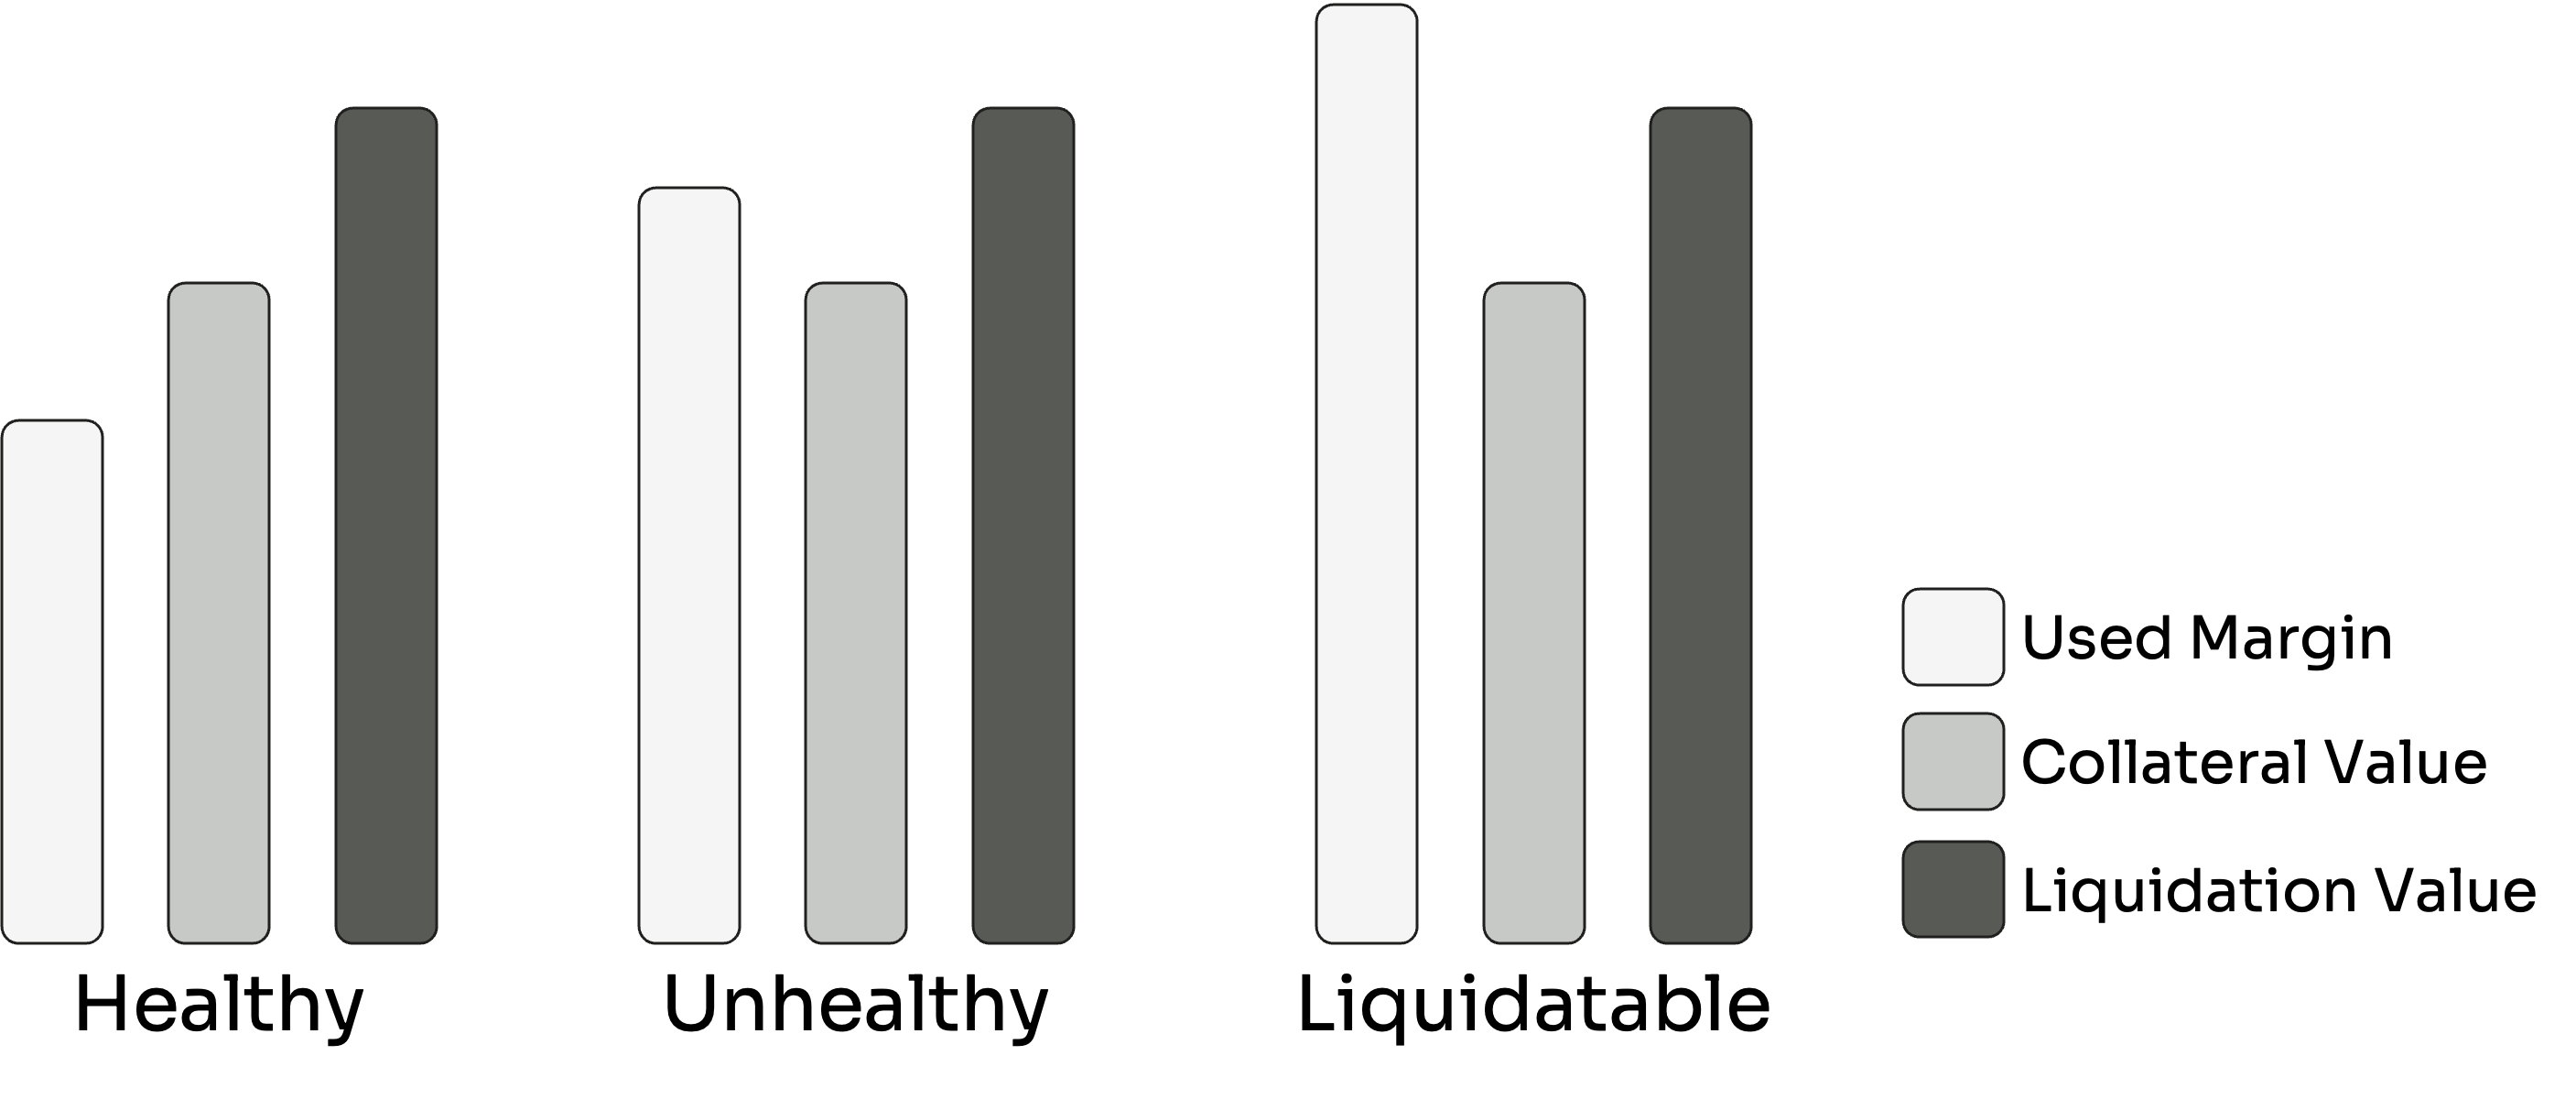
\includegraphics[width=0.4\textwidth]{images/Health-States.png}
    \caption{Margin Account health states. \label{fig:health-states}}
    \Description{The Margin Account health states.}
\end{figure}

\begin{enumerate}
    \item \textsc{Healthy state:} The Account is in a healthy state if the used margin is smaller than the Collateral Value:
        \begin{equation}
            um < v_{coll}
        \end{equation}

        No account actions are restricted for Accounts in a healthy state, as long as the Account is still healthy at the end the action.
    \item \textsc{Unhealthy state:} The Account is in an unhealthy state if the used margin is smaller than the Collateral Value but bigger than the Liquidation Value:
        \begin{equation}
            v_{coll} < um < v_{liq}
        \end{equation}
        
        Accounts in the unhealthy state can only be de-risked by or reducing the open position, or adding more collateral assets.
        It is not possible to withdraw any asset or to increase the open position.
    \item \textsc{Liquidatable state:} The Account is in a liquidatable state if the used margin is smaller than the Liquidation Value:
        \begin{equation}
            v_{liq} < um
        \end{equation}
        
        When an account is in the liquidatable state, anyone can trigger a margin call.
        The Account is now frozen and a liquidation process of the Account starts.
        The liquidation ends when either the Account is brought back in a healthy state, or all assets are liquidated.
\end{enumerate}

\subsection{Multi-Asset}
\label{subsec:multi-asset}
The owner of the Account can deposit and withdraw a multitude of collateral assets.
The list of assets that can be deposited in Arcadia Accounts is continuously being expanded, thanks to the modular architecture of the Arcadia Registry (see Paragraph \ref{subsec:modular-pricing-logic}).

By allowing multiple assets to be deposited within a single Account, users, institutions and protocols can build diversified portfolios and complex strategies.

That does however not mean that Creditors have to be exposed to an ever increasing list of assets.
Creditors can limit which assets are allowed as collateral in Accounts of their Debtors,
and set appropriate risk parameters for the assets they allow (see Paragraph \ref{subsec:creditor-specific-cisk-parameters}).

New assets that can be deposited into Accounts are by default not accepted for a Creditor.
Only if the Creditor explicitly allows the asset, can their Debtors use it as collateral.

\subsection{Token Standard Agnostic}
Accounts are token-standard agnostic, meaning not only typical ERC-20 tokens can be deposited,
Also assets complying with other standards, such as ERC-721 (”NFTs”, such as Uniswap V3 LP positions) and ERC-1155 assets can be held in an Arcadia Account.

That does however not mean that because ERC-721 is supported, all implementations of ERC-721 are supported.
As mentioned in Paragraph \ref{subsec:multi-asset}, each individual asset (individual contract address and, if applicable, token Id)
must be allowed by the Registry and secondly be accepted by the Creditor before a Debtor can use it as collateral.

Because the Account logic is upgradable, see Paragraph \ref{subsec:upgradeability}, even future token standards can be supported by Arcadia Accounts,
if both the Account owner and Creditor agree.

\subsection{Upgradeability}
\label{subsec:upgradeability}

Arcadia Accounts are based on the ERC-1967 standard for proxy contracts.
Each Account contract points to a certain Account logic contract.
It is the logic contract that implements the features to: deposit/withdraw assets, do flash actions, manage assets, authorise delegations...

Different implementations of the Account logic can (co)exist and each implementation is uniquely identified with a specific version in the Account Factory,
as illustrated in Figure \ref{fig:proxy-accounts}.
The Arcadia team can periodically push a new version to the Arcadia Factory, which might add new features, extend logic, or implement other improvements.

\begin{figure}
    \centering
    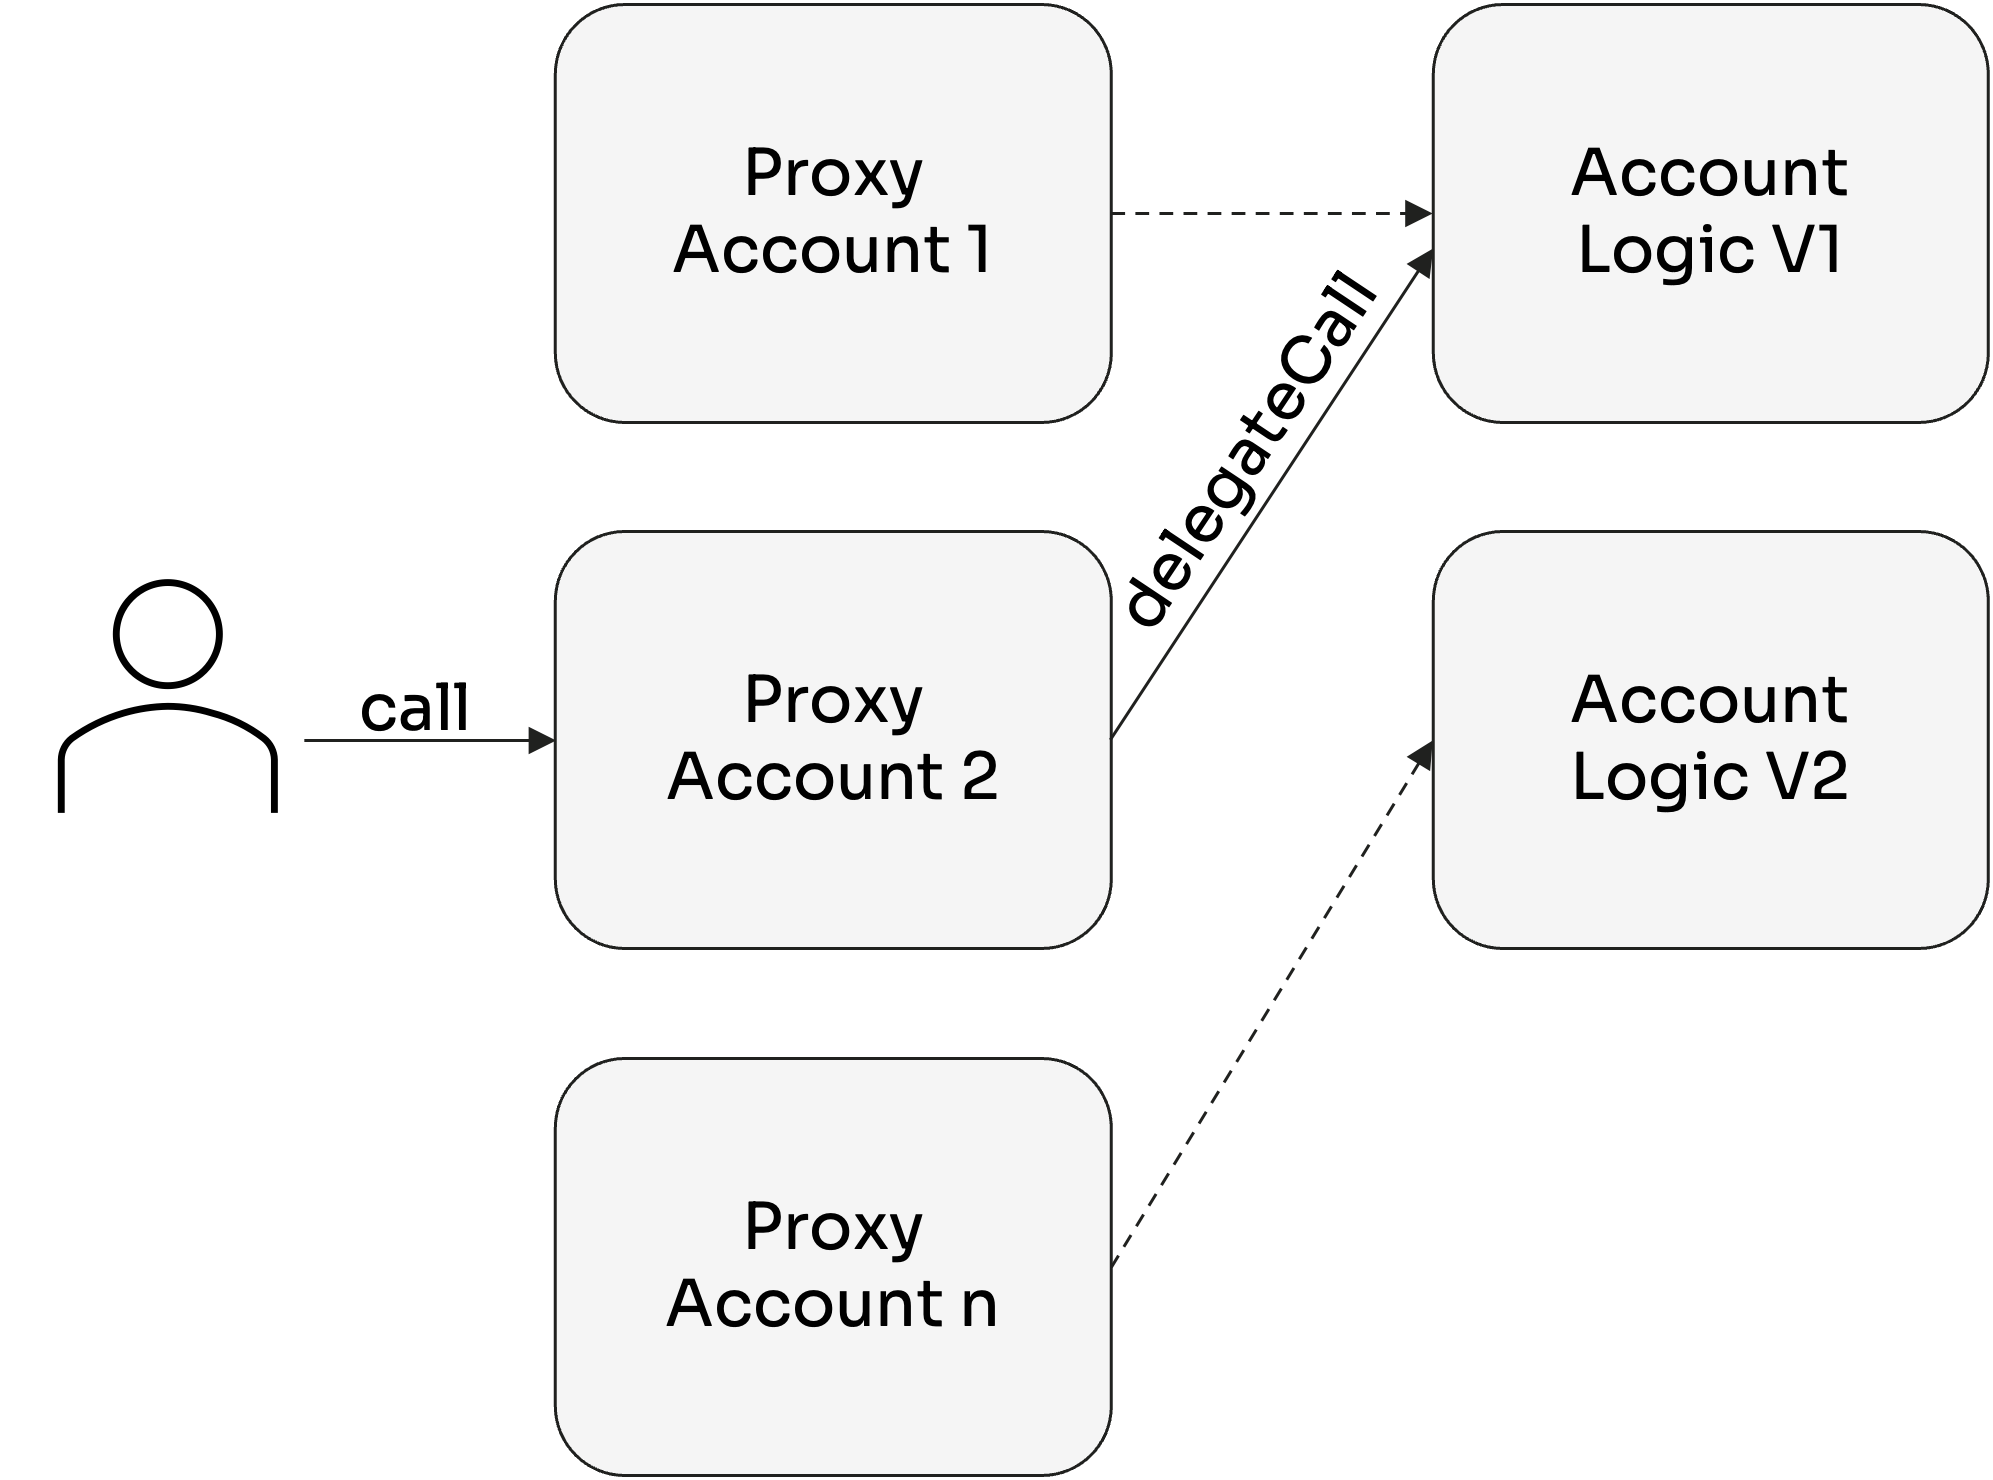
\includegraphics[width=0.45\textwidth]{images/Proxy-Accounts.png}
    \caption{Arcadia Proxy Accounts and Account Logic Versions. \label{fig:proxy-accounts}}
    \Description{Shematic of the Proxy Accounts and their relation to the Account Logic.}
\end{figure}

Creditors can determine which Account logic versions are allowed to be used by their Debtors.
As such, they can block version with certain features or highly-customized Account logic can be implemented for Creditor-specific versions should this be required.

The Account logic is upgradable, enabling existing accounts to make use of newly introduced features in a new Account version if they wish.
Upgrading Account logic is always on an opt-in basis, it can never be enforced by the Arcadia protocol.
The Accounts can only be upgraded to a different version if both the Account owner and the Creditor (if a margin account is opened) accept the specific version.

When users upgrade their Accounts, they don't have to migrate any assets or close liabilities and the Accounts keeps the same contract address.

\subsection{Composable}
Arcadia Accounts themselves are according to the ERC-721 standard and can thus be represented as a single asset on-chain.
This means that Accounts are fully composable with existing infrastructure and can be displayed in existing portfolio trackers as such (eg. Zapper, OpenSea, DeBank, …).

An Arcadia Account can be transferred (or sold!) as a whole, including all assets and liabilities, just like you are used to transferring NFTs.

\subsection{Flash Actions}
% Add image illustrating flash actions?
Flash Actions (or optimistic Actions or flash accounting) expands on the concept of flashloans, and are only possible thanks to a unique property of smart contracts: atomicity\cite{xie2022towards}.
Just as with flashloans, each step of the Flash Action must be successful or the transaction as a whole fails.

The final health check of the Account ("Can the assets cover all liabilities?") is done at the very end of the transaction.
This allows the Account Owner to temporary bring the Account in an under-collateralized (or even non-collateralized state) without the risk on bad debt for any Creditor.
Since if the Account is not brought back into a healthy state during the transaction, the final health check fails and thanks to atomicity the whole transaction fails.

This gives Account Owners unprecedented flexibility to manage assets and liabilities.
In a fully permissionless way they can chain the following actions together in one Flash Action:
\begin{itemize}
    \item A margin Account can be opened for a new Creditor, if the new Creditor is approved by the Account Owner.
    \item The Creditor can execute arbitrary logic (e.g. give a flashloan).
    \item The Account owner can optimistically withdraw assets from the Account.
    \item The Account owner can transfer assets from his own wallet to the Account or external logic.
    \item The Account owner can execute arbitrary external logic, where they uses the assets (loaned, withdrawn or transferred) to interact with multiple DeFi protocols to swap, stake, claim...
    \item The Account owner can deposit recipient tokens back into the Account.
\end{itemize}
The only requirement is that the Account is in a healthy state at the very end of the Flash Action.

Flash Actions are a very powerful tool that has no equal in traditional finance.
We will list a few examples how Flash Actions from an Arcadia Account can be used out of the box (the list is far from exhaustive).
Keep in mind that all of these actions can be done, even if the assets in the Account are used to secure liabilities.

\begin{itemize}
    \item Rebalance whole portfolios, swapping a portfolio of n different assets directly to a new portfolio of m different assets.
    \item Refinance liabilities (change to a different Creditors), without the need to sell any collateral.
    \item Stake or provide liquidity on approved DeFi protocols.
    External protocols used in this context will need to provide a receipt token which must be allowed as collateral as well within the Arcadia protocol.
    Examples can be providing liquidity on Aave (receiving approved aTokens), depositing assets on Yearn (receiving approved yTokens), …
    \item Change ranges for Uniswap V3 LP. Contrary to Uni V2 and similar AMMs, Uni V3 positions are meant to be more actively managed in terms of liquidity ranges.
    Users that deposit Uni V3 positions in their Arcadia Accounts will have the ability to change those liquidity ranges without having to withdraw their tokens first.
    \item Claim airdrops that depend on address-owned tokens. Arcadia Accounts will feature “flash withdrawals”.
    This feature can be used by the Account owner to claim airdrops using assets under collateral within their Arcadia Account, without having to close DeFi positions to withdraw their tokens first.
    \item ...
\end{itemize}

\subsection{Account Abstraction Ready}
\label{subsec:account-abstraction-ready}
As mentioned in Paragraph \ref{subsubsec:end-user-complexity}, account abstraction is an important step forward in reducing end-user complexities and decreasing operational risks.

At the time of writing this paper, there is no social consensus yet about which standard to use for account abstraction within the Ethereum ecosystem.
Hence Arcadia Accounts will initially not be "real abstract accounts" and still require an EOA (Externally Owned Account) owning and controlling the actions of the Arcadia Account.
Instead the Arcadia Accounts are "Account Abstraction ready".

Still some key features of account abstraction are implemented in a non-standardized form.
Most notable the ability to bundle multiple actions, and the ability to set an entry point that can do operations on behalf of the account owner.

The Arcadia Accounts are implemented in such a way that if at some point account abstraction is standardized, they can be easily modified to adhere to the agreed upon standard.
Even users with existing accounts can (if they want) upgrade their Accounts to this new version with full Account Abstraction, as explained in Paragraph \ref{subsec:upgradeability}.

\subsection{Intent Ready}
We truly believe in the benefits intent based architectures bring for end-users,
especially for collateral and asset management.

But similarly to what we said in Paragraph \ref{subsec:account-abstraction-ready} about Account Abstraction,
there is, at the time of writing this paper, no generalized infrastructure or standardization for intents within the Ethereum ecosystem yet.

The Arcadia Accounts are however designed to be "intent ready".
They will initially work with a non-standard single solver for intent based actions, with certain off-chain dependencies.

And secondly, the Arcadia Account require little modifications to support "full intents" as soon as the required infra/standard is available.
This would again require an upgrade of the Accounts logic as described in Paragraph \ref{subsec:upgradeability}.

\subsection{Automated Asset Management}
Account owners can appoint one or more Asset Managers, including external smart contracts, which can take actions on behave of the Account owner.

The Asset Manager is a fully trusted role, and should be used with care.
No Account owner should set an Asset Manager which they doesn't trust with their funds.

The Asset Manager has multiple use-cases, a few examples are (non exhaustive list):
\begin{itemize}
    \item Automate strategies via programmatically controlled EOA.
    \item Automate certain account actions (rebalancing, decrease leverage, stop losses...) with keeper networks.
    \item Set an Entry point for user operations (abstracted transactions).
    \item Delegate asset management to third parties.
\end{itemize}

\section{Arcadia Creditor}
\label{sec:arcadia-creditor}
An Arcadia Creditor is a (set of) smart contract(s),
that does the accounting of the open position(s) between one or more Debtor(s) and one or more Creditor(s),
and where all open positions are fully secured by the collateral held in Arcadia Accounts,
owned by each of the Debtors.

Examples of Creditors can be implementations of peer-to-peer lending protocols, peer-to-pool lending, perpetual futures contracts, options contracts, escrow services...
An Arcadia Creditor can be implemented for basically every financial contract or protocol where a party has, or can have, liabilities.

\subsection{Generalized Creditor}
Since the Arcadia Finance Technology Stack is open and permissionless,
every financial contract or protocol with one or more Debtors,
can build on top of the Arcadia Finance Technology Stack.

Protocols that whish to do so, only have to implement the Arcadia Creditor interface
and are immediately compatible with the Arcadia Registry and Arcadia Accounts.

Next to the advantages as laid out in Paragraph \ref{subsec:new-architectures},
this means they don't have to implement any logic for collateral management and margin calculations themselves.
This greatly reduces smart contract development time, auditing costs and go to market times.

In the next paragraphs we will discuss the most important features of the Arcadia Creditor interface.

\subsubsection{Accounting Liabilities}
Most important is the correct accounting of the open positions of the Debtors.
As explained in Paragraph \ref{subsubsec:margin-account-health-states},
the open position is used for the margin calculations to determine the health state of the Arcadia Account of Debtor.
In turn, this guarantees that all liabilities can be paid back to the Creditor.

A Creditor must denominate their liabilities in a certain numeraire.
This represents the unit of accounting, for example USD, USDC or ETH.

The Arcadia Account of the Debtors will use the same numeraire for the margin calculations.

\subsubsection{Risk Management}
The owner of a Creditor must set a Risk Manager.
The Risk manager can be both an EOA or a smart contract.

The Risk Manager is responsible for setting and maintaining the correct Collateral and Liquidation Factors for all assets that can be used by Debtors as collateral.
Next to these factors, the Risk Manager also sets the exposure limits against each individual asset. 

In short, it protects the Creditor against market and other risks, and ensures the credit risk borne by the Creditor remains acceptable.

\subsubsection{Allowed Account Versions}
As explained in paragraph \ref{subsec:upgradeability}, multiple Account versions can coexist.

Each Creditor can approve one or more of these Account versions,
meaning that only Accounts with an approved version are able to open positions with the respective Creditor.

\subsubsection{Liquidations}
Every Creditor must ensure that a suitable liquidation flow is foreseen in case an Account's health state drops to the liquidatable state,
as explained in Paragraph \ref{subsubsec:margin-account-health-states}.

The Arcadia team already developed a robust liquidation flow which can be re-used by other Creditors,
which is further described in Paragraph \ref{subsubsec:liquidations}.

\subsection{Arcadia Lending Pools}
The Arcadia Lending Pools are just one example of an implementation of an Arcadia Creditor.

Since the Arcadia Lending Pools are an implementation of the Arcadia Creditor,
they come with the features as mentioned in Paragraph \ref{sec:arcadia-creditor}.

An Arcadia Lending Pool is a peer-to-pool lending protocol, developed by the Arcadia team.
On a conceptual level, it consists of a two-sided lending market between liquidity providers and borrowers.

Next to that, the Lending Pools also come with a number of innovations compared to other peer-to-pool lending protocols.

\subsubsection{Interests}
Arcadia Lending will use a variable interest rate, depending on the utilization rate of the underlying Lending Pool.

Every-time a user interacts with the Lending Pool (depositing/withdrawing liquidity, taking/repaying debt),
the accounting logic for interest payments is triggered and the new interest rate is calculated.
Interests are continuously compounding.

The ERC-4626 standard is used to represent both the open positions of Debtors (see Paragraph \ref{subsubsec:accounting-liabilities}),
and the yield bearing positions of liquidity providers (see Paragraph \ref{subsubsec:accounting-liquidity}).
Using the ERC-4626 standard makes the accounting logic gas efficient and ensures composability with existing protocols and infrastructure.

\subsubsection{Accounting Liabilities}
\label{subsubsec:accounting-liabilities}
When a Debtor borrows from the Lending Pool,
an ERC-4626 token (the debt token or dToken) will be minted to the Debtor's Arcadia Account.
The dTokens tokens are not transferable.

The interests on all debt are automatically and continuously accruing via the ERC-4626 standard.

\subsubsection{Tranches}
Each Lending Pool consists of one or more risk Tranches.
A Tranche is a slice of the total liquidity in the pool, with a different risk-reward profile compared to other Tranches.

For example, the most Junior Tranche receives a larger relative share of the interest payments and a larger relative share of the liquidation penalties,
but is slashed first should any bad debt occur.

Similarly, a more Senior Tranche may have lower yields through interests and liquidations,
but will only be slashed due to bad debt as soon as each more Junior Tranche is completely slashed.

With some game-theory in mind, the overall risk-reward of a more Junior Tranche will be higher than of a more Senior Tranche.

The main advantage of risk Tranches is that Liquidity Providers with different risk-reward preferences can provide liquidity,
but that all liquidity is still pooled in the same underlying Lending Pool.
Not fragmenting the liquidity over different pools results in deeper liquidity for the borrowers and more stable interest rates.

\subsubsection{Accounting Liquidity}
\label{subsubsec:accounting-liquidity}
Anyone who owns the underlying asset of the Lending Pool, can deposit liquidity via one of the Tranches.

When a Liquidity Provider (LP) deposits liquidity, they receive an ERC-4626 yield bearing token (ybToken).
Each Tranche will have its own ERC-4626 token.

The Lending Pool will do the accounting to keep track of how much liquidity is owned by each Tranche,
while the tranches in turn will do the accounting of how much of that liquidity is owned by their respective LPs.
A schematic of an Arcadia Lending Pool with Tranches is illustrated in Figure \ref{fig:tranches}.

\begin{figure}
    \centering
    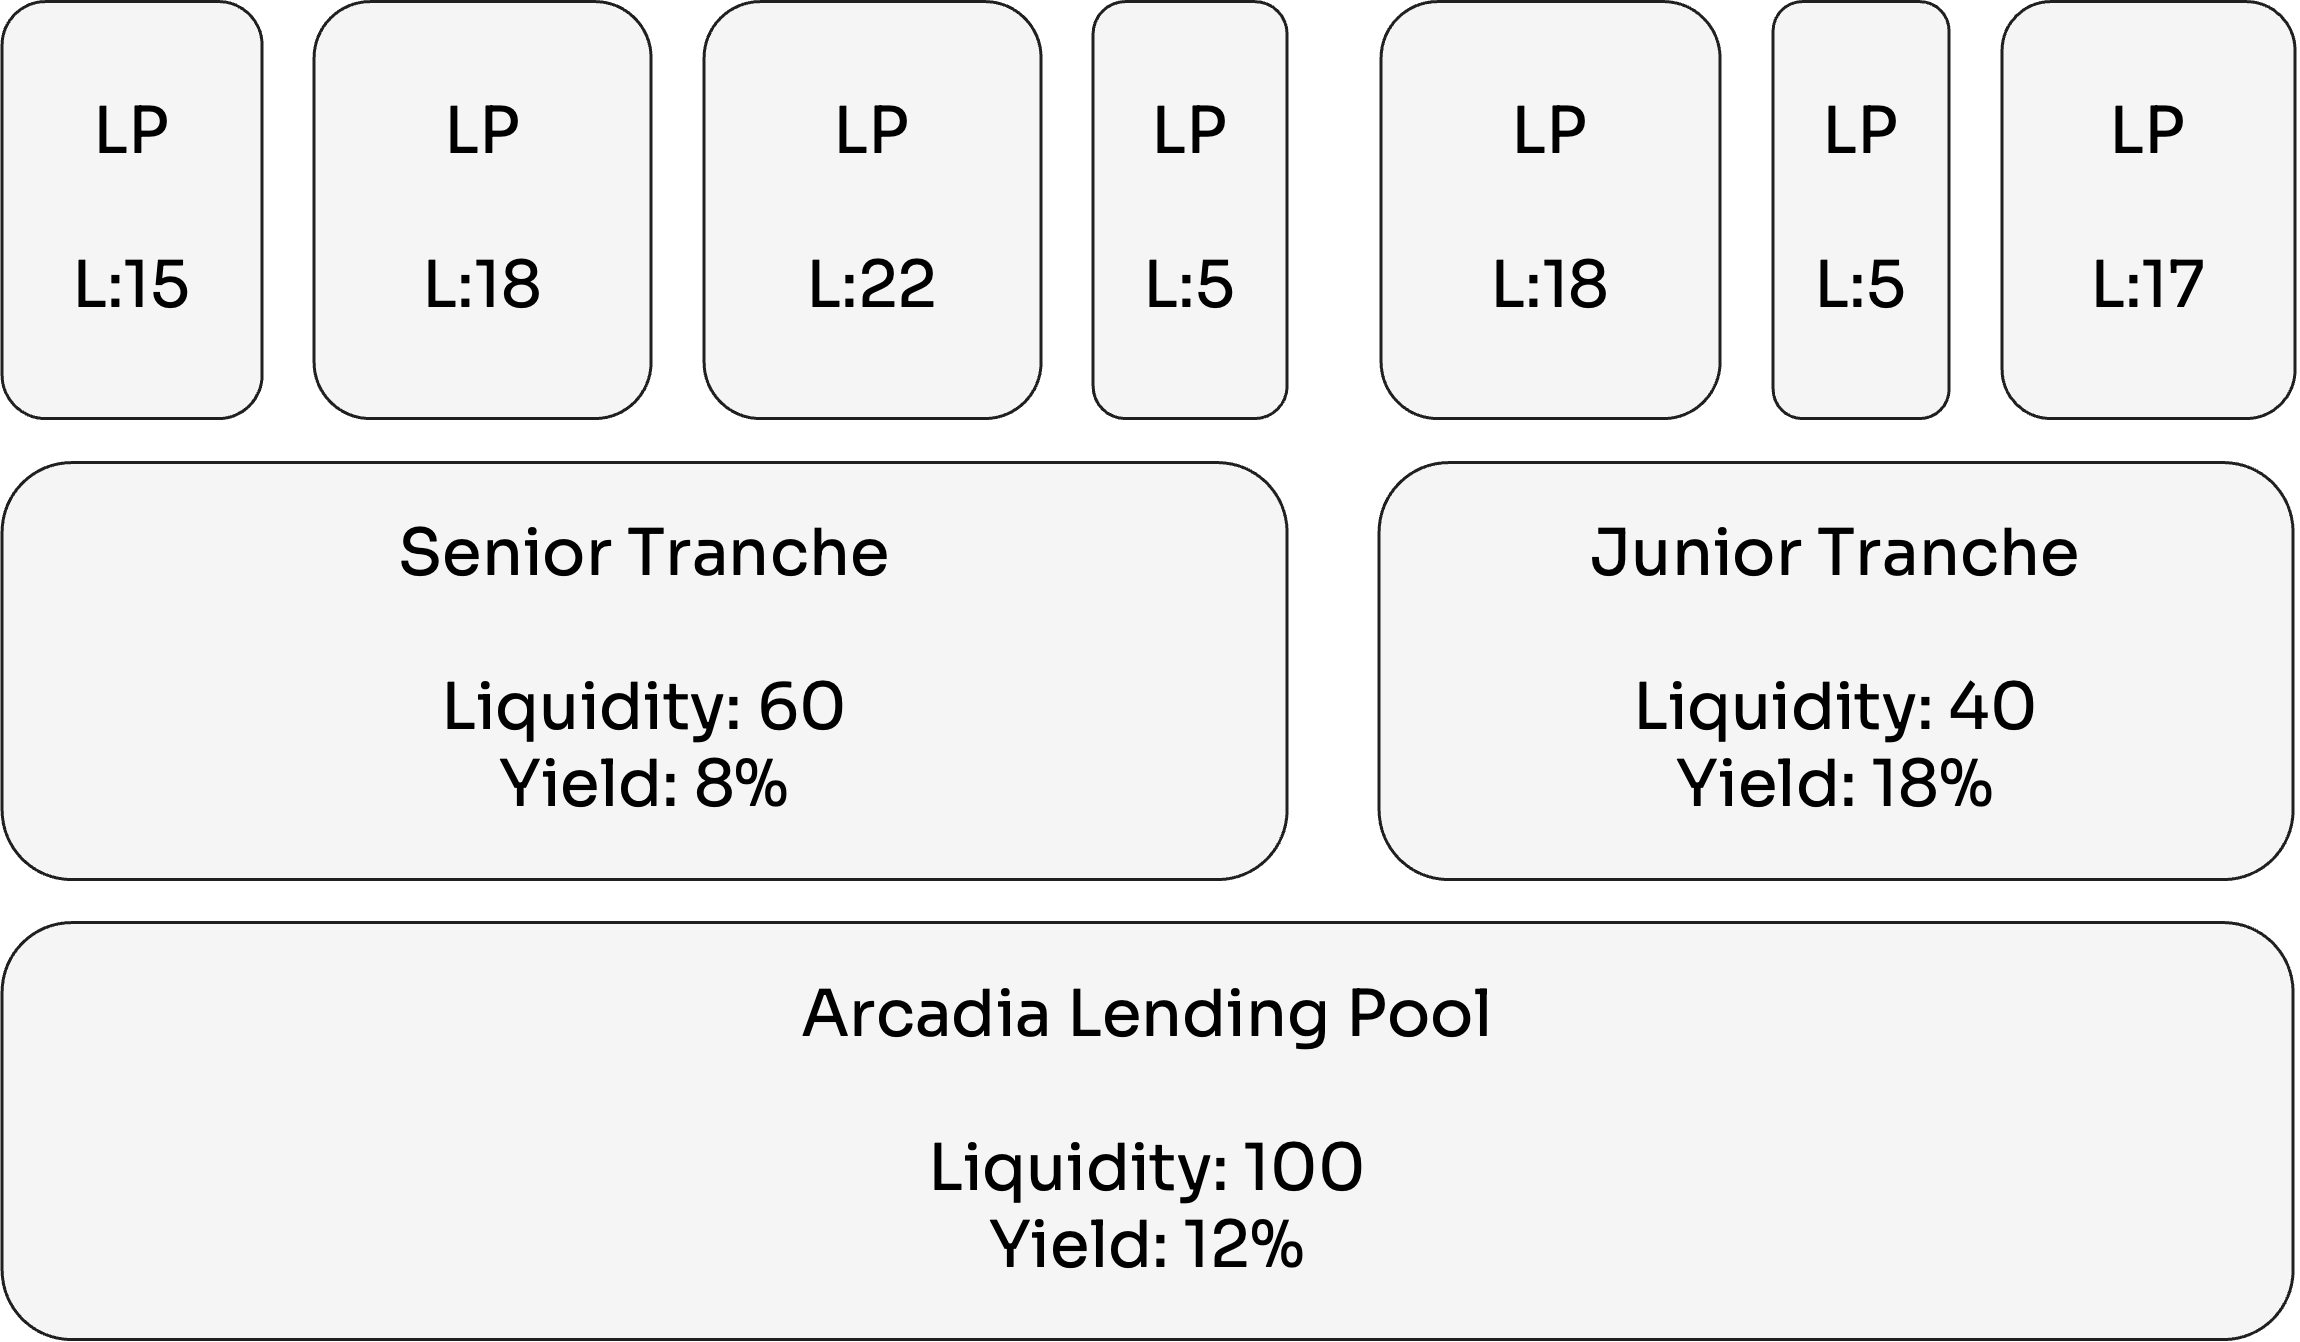
\includegraphics[width=0.45\textwidth]{images/Tranches.png}
    \caption{Arcadia Lending Pool with two Tranches. \label{fig:tranches}}
    \Description{A schematic of the Arcadia Lending Pool, two Tranches and their LPs.}
\end{figure}

Yield earned through interests and liquidation fees is divided over the different Tranches
(more Junior tranches will earns a bigger relative share of the yield).
Via the ERC-4626 standard, the yield is further pro-rata distributed to the LPs of the Tranches.

\subsubsection{Liquidations}
\label{subsubsec:liquidations}
Liquidations for Arcadia Lending Pool are conducted via a three-step process using a Gradual Dutch Auction.

Initially, anyone can initiate the liquidation of an Account that falls below the liquidatable health threshold,
receiving a reward for doing so.

After the liquidation is initiated, a Gradual Dutch Auction starts where the Account's asset prices gradually decrease until a buyer,
typically an MEV searcher, steps in and places an atomic bid.
The process allows for partial liquidations to reduce market impact.

Anyone can end the auction, and also receives a reward for doing so, if any if the following conditions are met:
\begin{itemize}
    \item The Account is back in a healthy state.
    \item All debt is repaid.
    \item All collateral assets are sold.
    \item A certain amount of time (set by the Lending Pool) has passed.
\end{itemize}

After the auction is successfully ended, the liquidation is settled.
There are three different scenarios, as illustrated in Figure \ref{fig:liquidation-settlement}, how a liquidation can be settled,
depending on the total proceeds of the auction relative to the debt and liquidation penalties:
\begin{enumerate}
    \item If the auction proceeds are less than the debt,
    the shortfall is covered by the Junior Tranche's tokens.
    \item If the auction proceeds exceed the debt but is under the debt plus liquidation penalty,
    the surplus is shared between Arcadia's treasury and the most Junior Tranche.
    \item If the auction proceeds surpass the debt and the liquidation penalty cap,
    excess funds after penalty distribution are returned to the Account's original owner.
\end{enumerate}

\begin{figure}
    \centering
    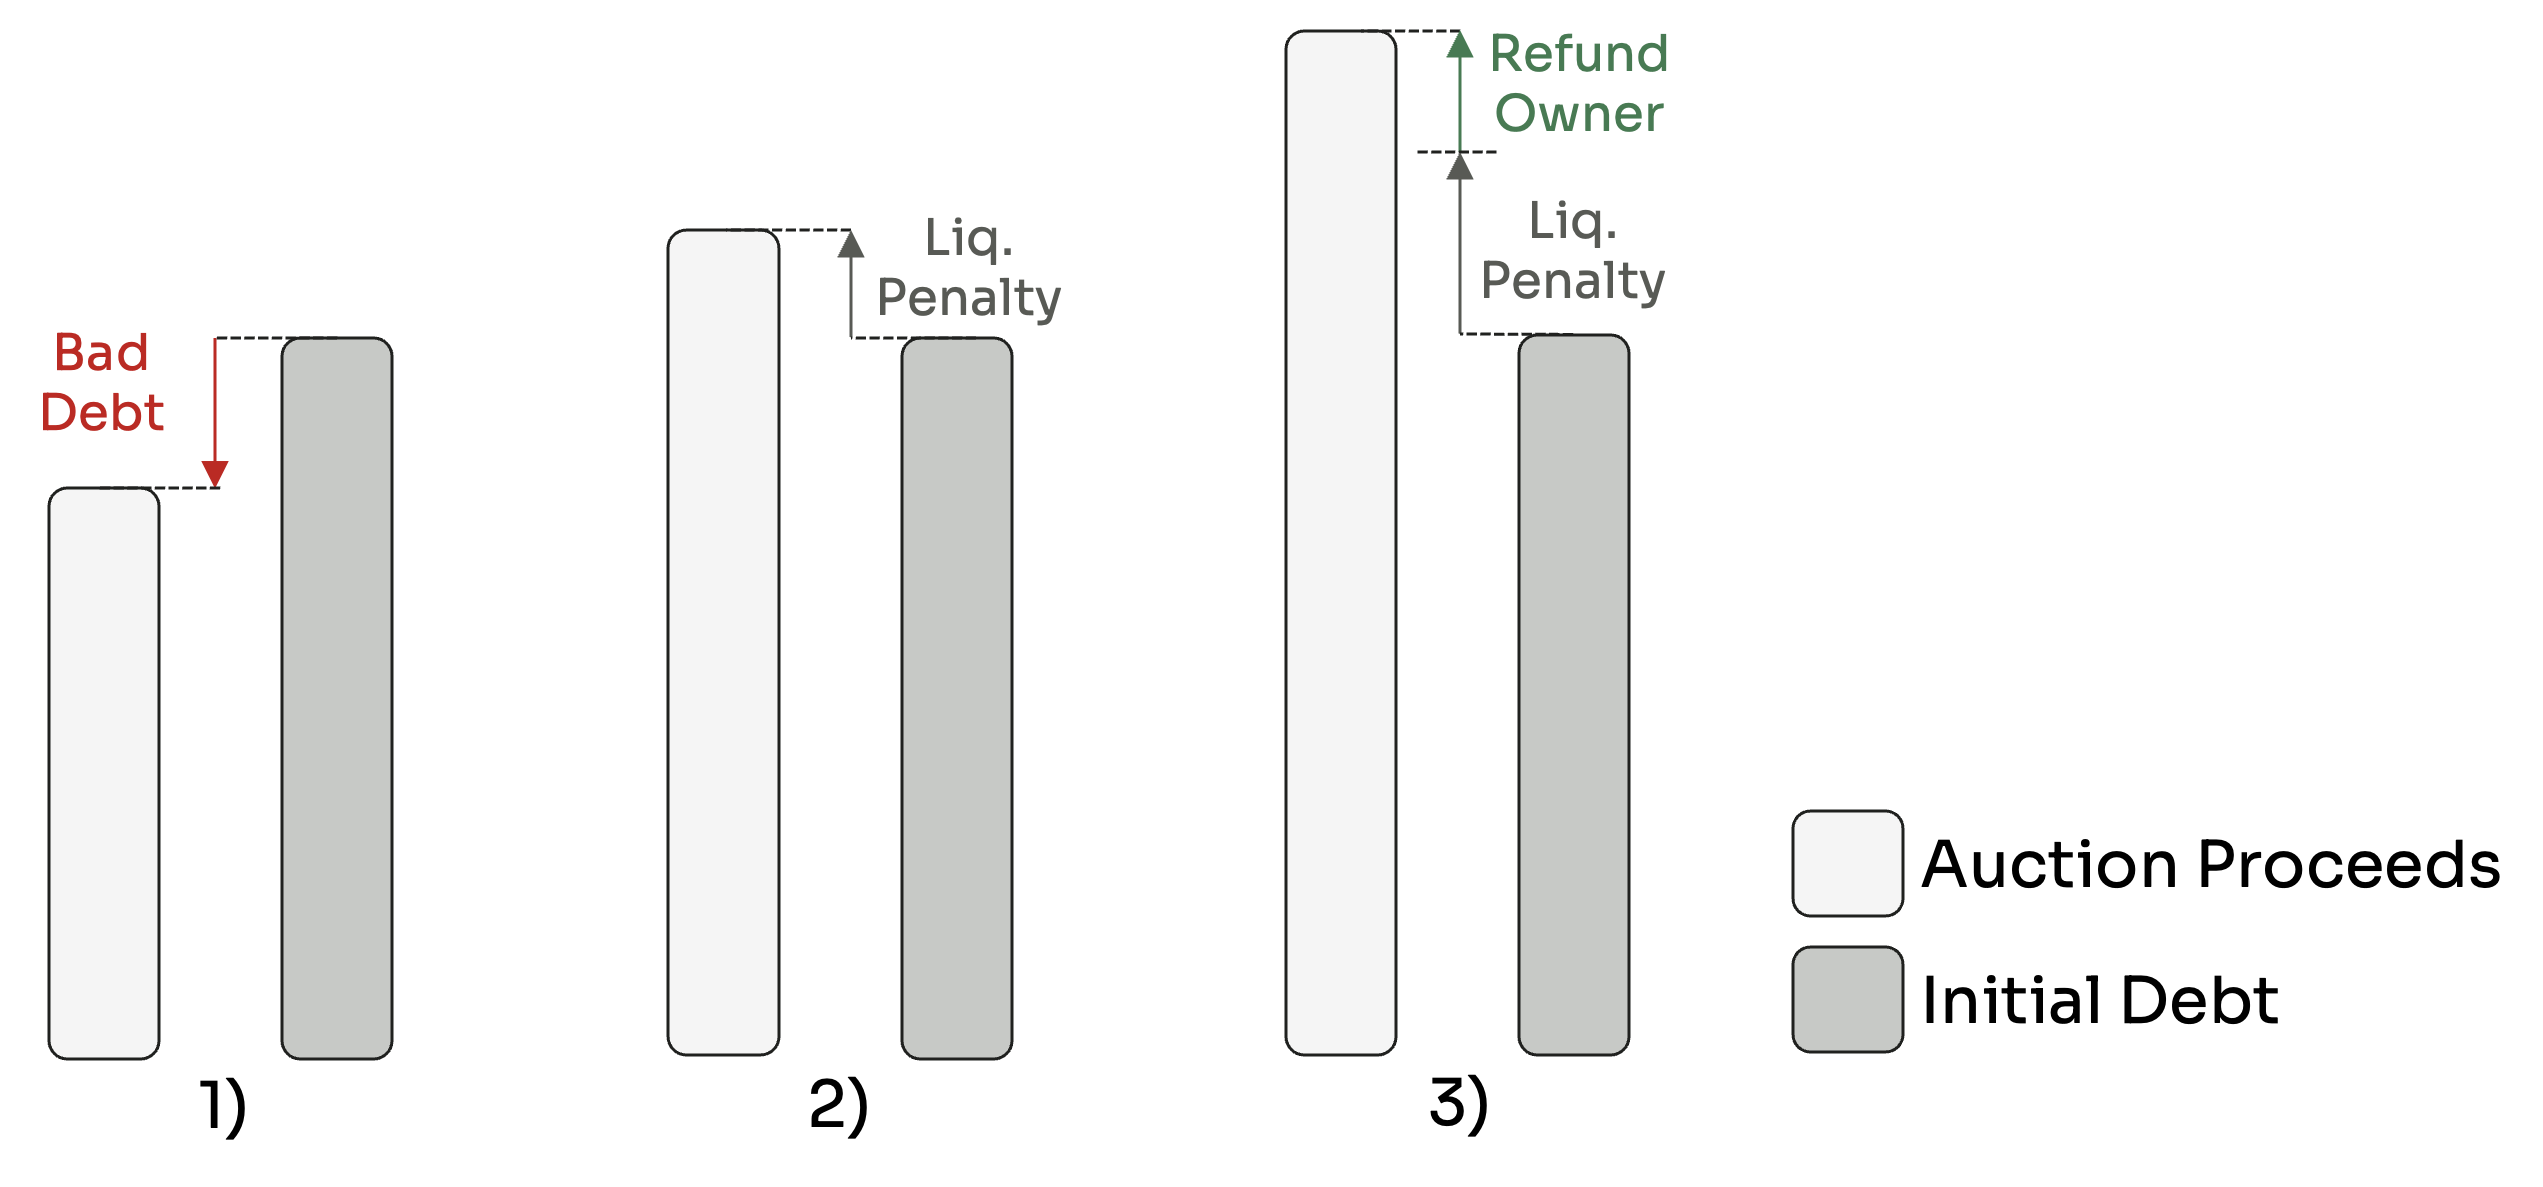
\includegraphics[width=0.45\textwidth]{images/Liquidation-Settlement.png}
    \caption{Liquidation Settlement scenarios. \label{fig:liquidation-settlement}}
    \Description{An illustration of the three different Liquidation Settlement scenarios.}
\end{figure}

\balance
\section{Summary}
\label{sec:summary}
In conclusion, this paper has explored the development and implementation of the Arcadia Finance Technology Stack:
A shared standardized and permissionless layer with battle-tested logic for collateral management and margined positions,
on top of which financial protocols can build their application specific financial contracts.

By leveraging this technology stack, protocols can streamline their development processes, reducing both time and potential bugs,
allowing them to concentrate on refining their core logic.
Simultaneously, users benefit from the simplicity of managing on-chain portfolios through a single Arcadia Account, minimizing risks,
and significantly enhancing the overall user experience.

In closing, we invite further exploration and collaboration to unlock the full potential of DeFi and contribute to the ongoing evolution of the financial system.

\section*{Disclaimer}
This document is intended for general informational purposes only and should not be construed as investment advice or
a recommendation to buy or sell any investments.
The views expressed herein represent the current opinions of the authors and are not presented on behalf of Arcadia Finance, Pragma Labs, or their affiliates.
The opinions conveyed do not necessarily align with those of Arcadia Finance, Pragma Labs, their affiliates, or associated individuals,
and they may be subject to change without prior updates.

\bibliographystyle{ACM-Reference-Format}
\bibliography{main}

\end{document}

\endinput
